\documentclass[11pt,a4paper,final]{article} 
\usepackage[english, russian]{babel}
\usepackage[final]{pdfpages}
\usepackage{textcomp,enumitem}
\usepackage{amsmath,amsthm,amssymb}
\usepackage{fancyhdr}
\usepackage{upgreek}
\usepackage{tipa}
\usepackage{tikz}
\usepackage{amsfonts}
\usepackage{caption}
\usepackage{subcaption}
\usepackage{float}
\usepackage{graphics}
\usepackage{pgfplots}
\usepackage{indentfirst}
\usepackage[unicode, pdftex, colorlinks, urlcolor=blue]{hyperref}
\usepackage{pdflscape}
\usepackage[T2A]{fontenc}
\usepackage[utf8]{inputenc} 
\usepackage[left=2cm,right=2cm,top=2cm,bottom=2cm,bindingo ffset=0cm, 
%showframe
]{geometry}
\usepackage{multirow}
\usepackage{capt-of}
\usepackage{needspace}
\usepackage{amsmath,amssymb,cmap,pgfplots,pgfplotstable}

\usetikzlibrary{arrows,calc,intersections}
\addto\captionsrussian{\def\refname{}}
\pgfplotsset{compat=newest}
\pgfplotsset{compat=1.9}
\linespread{1.5}
\pagestyle{plain}
\begin{document}
	%\thispagestyle{empty}
	\begin{center}
		{\large МИНОБРНАУКИ РОССИИ}
		\par
		\vspace{8pt}
		{\large ФЕДЕРАЛЬНОЕ ГОСУДАРСТВЕННОЕ БЮДЖЕТНОЕ ОБРАЗОВАТЕЛЬНОЕ УЧРЕЖДЕНИЕ}
		\vspace{7pt} 
		{\large ВЫСШЕГО ПРОФЕССИОНАЛЬНОГО ОБРАЗОВАНИЯ}
		
		\vspace{3pt} 
		{\Large \bf <<САНКТ-ПЕТЕРБУРГСКИЙ ПОЛИТЕХНИЧЕСКИЙ УНИВЕРСИТЕТ ПЕТРА ВЕЛИКОГО>>}
		
		\vspace{1pt}
		{\Large Институт Компьютерных наук и кибербезопастности}
		
		\vspace{1pt} 
		{\Large Направление 02.03.01 Математика и компьютерные науки}
		
		\vspace{1pt} 
		{\Large Высшая школа технологий искусственного интеллекта}
		
		\vspace{75pt} 
		{\large ОТЧЕТ ПО ЛАБОРАТОРНОЙ РАБОТЕ №2 ПО ДИСИПЛИНЕ ТЕОРИЯ АЛГОРИТМОВ}
		{\large }\\
		
		\vspace{10pt}
		{\Huge \bf Синтез функциональной схемы часов} \\
		\vspace{10pt}
		{\Huge \bf Вариант 39}
	\end{center}
	
	\vspace{110pt} 
	\hspace{1cm}
	{\large Обучающийся: \ \ \ \underline{\ \ \ \ \ \ \ \ \ \ \ \ \ \ \ \ \ \ \ \ \ \ \ \ \ \ \ \ \ \ }
		\hspace {2cm} Санько В. В.} 
	
	\vspace{10pt} 
	\hspace{1cm}
	{\large Руководитель: \ \ \ \underline{\ \ \ \ \ \ \ \ \ \ \ \ \ \ \ \ \ \ \ \ \ \ \ \ \ \ \ \ \ } 
		\hspace {2.25cm} Востров А. В.}
	
	\vspace{40pt} 
	\begin{flushright}
		{<<\underline{\ \ \ \ \ \ \ \ }>>\underline{\ \ \ \ \ \ \ \ \ \ \ \ \ \ \ \ \ \ \ \ \ }
			20\underline{\ \ \ \ \ }г.}
	\end{flushright}
	
	\vspace{80pt} 
	\begin{center}
		{\large Санкт-Петербург, 2026}
	\end{center}
	\thispagestyle{empty}
	
	
	\newpage
	\tableofcontents
	
	\newpage
	\section* {Введение}
	\addcontentsline{toc}{section}{Введение}
	Электронные часы представляют собой сложную цифровую систему, предназначенную для точного отсчёта и отображение времени. Данная работа посвящена синтезу функциональной схемы таких часов на основе конечно-автоматной модели управления. В рамках проекта рассматриваются основные компоненты устройства: система отображения на сегментных индикаторах, счётчики времени с генератором тактовых импульсов, а также управляющий конечный автомат, обрабатывающий действия пользователя.
	
	 В итоге была проведена детальная разработка структурно-функциональной схемы, демонстрирующей основные механизмы построения дискретных управляющих систем
	 
	 \newpage
	 \section{Постановка задачи}
	 
	 В соответствии с вариантом 110012221 необходимо реализовать часы удовлетворяюзие следующим условиям:
	 
	 \begin{itemize}
	 	\item A = 1 — отображение и корректировка секунд.
	 	\item B = 1 — два счетчика времени в разных часовых поясах, различаются только на n часов.
	 	\item C = 0 — корректировка десятков и единиц совместная.
	 	\item D = 0 — 12-часовой режим с индикацией a.m. / p.m.
	 	\item E = 1 — отключение индикаторов с целью экономии энергии присутствует.
	 	\item F = 2 — останов часов после состояния корректировки текущего времени.
	 	\item G = 2 — секундомер с фиксацией накопленного времени и возможностью продолжения отсчета.
	 	\item H = 2 — звуковая сигнализация каждые четверть часа в течение 1 секунды.
	 	\item I = 1 — будильник в течение 10 секунд с возможностью отключения режима.
	 \end{itemize}
	 
	 Для реализации указанного функционала требуется:
	 \begin{enumerate}
	 	\item Разработать граф управляющего конечного автомата, задающий логику работы всех режимов, и дать подробное описание его состояний, переходов и визуальной индикации.
	 	\item Построить общую структурную схему электронных часов, указав все необходимые управляющие микрокоманды (импульсные и потенциальные) и пояснив назначение каждого блока.
	 	\item Провести кодирование входных сигналов, выходных микрокоманд и внутренних состояний автомата.
	 	\item Выполнить минимизацию логических функций для блоков формирования состояний (F) и выходных потенциальных сигналов (FL) с помощью карт Карно.
	 \end{enumerate}
	 

	
	\newpage
	\section{Математическое описание}
	\subsection{Конечный автомат}
	Математическая модель дискретного устройства, которая описывается набором $A = (S, X, Z, s_0, \delta, \lambda)$, где 
	\begin{itemize}
		\item $S = \{s_0, s_1, s_2, ... , s_{15}\} \text{-- множество состояний}$
		\item $X = \{x_1, x_2\} \text{-- множество входных сигналов}$
		\item $Z = \{z_0, z_1, z_2, ... , z_7\} \text{-- множество выходных сигналов}$
		\item $s_0 \text{-- начальное состояние} $
		\item $\delta: S \times X \rightarrow S \text{-- функция переходов}$
		\item  $\lambda: S \times X \rightarrow Z \text{-- функция выходов}$
	\end{itemize}
	
	Конечный автомат работает в дискретные моменты времени. В момент времени $t=0$ автомат всегда будет находиться в начальном состоянии $s_0$.

	
	\subsection{Граф управляещего автомата часов}
	Граф управляещего конечного автомата электронных часов изображен на Рис. \ref{1:1}.
	
	\newpage % Переход на новую страницу
	\begin{landscape} % Начало альбомной ориентации
		\thispagestyle{empty} % (Опционально) Убирает номер страницы, чтобы было больше места
		
		\begin{figure}[p] % Параметр [p] означает "разместить на отдельной странице"
			\centering
			% Картинка растягивается по ширине или высоте, сохраняя пропорции
			% 0.95\textheight оставляет немного места для подписи снизу
			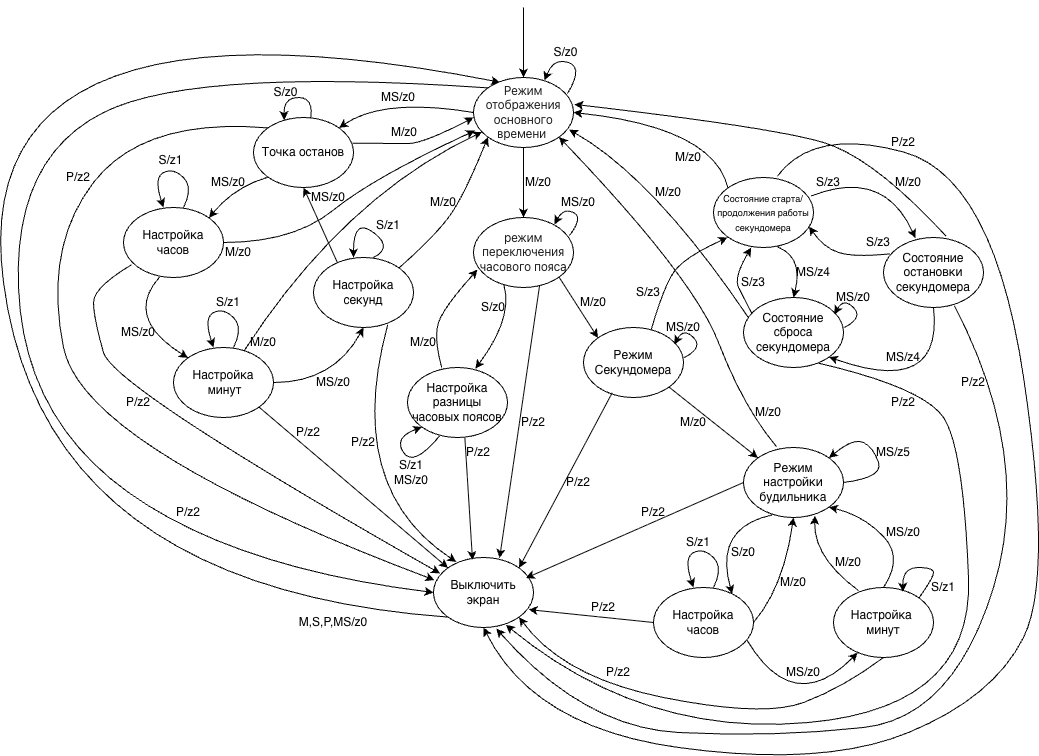
\includegraphics[width=1\linewidth, height=0.95\textheight, keepaspectratio]{img/113.png} 
			\caption{Граф конечного автомата часов}
			\label{1:1}
		\end{figure}
		
	\end{landscape} % Конец альбомной ориентации
	\newpage
	
	Стоит отметить, что из любой вершины графа по кнопке P осуществляется переход к вершине \texttt{Выключить экран} и из этой вершины по любой кнопке переход к \texttt{Дисплей}.
	
	
	\subsection{Таблицы для синтеза конечного автомата управления часами}
	
	
	\subsubsection*{1. Кодировка состояний \( S_i \rightarrow (q_1 q_2 q_3 q_4) \)}
	 Выделено 16 состояний автомата, все они перечислены в таблице \ref{tab1:0}:
	 \[
	 S = \{S_0, S_1, S_2, S_3, S_4, S_5, S_6, S_7, S_8, S_9, S_{10}, S_{11}, S_{12}, S_{13}, S_{14}, S_{15}\}
	 \]
	\begin{center}
		\captionof{table}{Кодировка состояний}
		\label{tab1:0}
		\begin{tabular}{|c|c|c|c|c|}
			\hline
			\( S_i \) & \( q_1 \) & \( q_2 \) & \( q_3 \) & \( q_4 \) \\
			\hline
			S0 & 0 & 0 & 0 & 0 \\
			S1 & 0 & 0 & 0 & 1 \\
			S2 & 0 & 0 & 1 & 0 \\
			S3 & 0 & 0 & 1 & 1 \\
			S4 & 0 & 1 & 0 & 0 \\
			S5 & 0 & 1 & 0 & 1 \\
			S6 & 0 & 1 & 1 & 0 \\
			S7 & 0 & 1 & 1 & 1 \\
			S8 & 1 & 0 & 0 & 0 \\
			S9 & 1 & 0 & 0 & 1 \\
			S10 & 1 & 0 & 1 & 0 \\
			S11 & 1 & 0 & 1 & 1 \\
			S12 & 1 & 1 & 0 & 0 \\
			S13 & 1 & 1 & 0 & 1 \\
			S14 & 1 & 1 & 1 & 0 \\
			S15 & 1 & 1 & 1 & 1 \\
			\hline
		\end{tabular}
	\end{center}
	
	\textbf{Пояснение состояний:}
	\begin{itemize}
		\item \textbf{S0 (Дисплей)} -- отображение текущего времени
		\item \textbf{S1 (Режим переключения часового пояса)} -- выбор/смена часового пояса
		\item \textbf{S2 (Настройка разницы часовых поясов)} -- коррекция смещения пояса (часы)
		\item \textbf{S3 (Секундомер остановлен)} -- режим секундомера (пауза)
		\item \textbf{S4 (Секундомер запущен)} -- секундомер считает время
		\item \textbf{S5 (Секундомер стоп)} -- секундомер остановлен, время зафиксировано
		\item \textbf{S6 (Секундомер сброшен)} -- сброс показаний секундомера
		\item \textbf{S7 (Настройка будильника)} -- меню будильника (вкл/выкл)
		\item \textbf{S8 (Установка часов будильника)} -- коррекция часов будильника
		\item \textbf{S9 (Установка минут будильника)} -- коррекция минут будильника
		\item \textbf{S10 (Точка остановы)} -- управление ходом основных часов (RUN/STOP)
		\item \textbf{S11 (Настройка часов)} -- коррекция основных часов
		\item \textbf{S12 (Настройка минут)} -- коррекция основных минут
		\item \textbf{S13 (Настройка секунд)} -- коррекция основных секунд
		\item \textbf{S14 (Выключить экран)} -- экран отключён (экономия энергии)
		\item \textbf{S15 (Режим активного будильника)} -- сработал будильник
	\end{itemize}
	
	\subsubsection*{2. Кодировка входных сигналов (кнопок) \( X \rightarrow (x_1 x_2) \)}
	
	Входной алфавит конечного автомата состоит из 4 элементов: кнопки S, M, P MS, таблица \ref{tab2:0}.
	
	\begin{center}
		\captionof{table}{Входы конечного автомата}
		\label{tab2:0}
		\begin{tabular}{|c|c|c|}
			\hline
			Вход (In) & \( x_1 \) & \( x_2 \) \\
			\hline
			S & 0 & 0 \\
			M & 0 & 1 \\
			MS & 1 & 0 \\
			P & 1 & 1 \\
			\hline
		\end{tabular}
	\end{center}
	
	\subsubsection*{3. Выходы конечного автомата}
	
	Было введено множество выходных сигналов, таблица \ref{tab3:0}:
	\[
	Z = \{z_0, z_1, z_2, z_3, z_4, z_5, z_6, z_7\}
	\]
	
	\begin{center}
		\captionof{table}{Выходы конечного автомата}
		\label{tab3:0}
		\small
		\begin{tabular}{|c|l|}
			\hline
			Обозначение & Расшифровка \\
			\hline
			\(z_0\) & Нейтральный сигнал (нет действий) \\
			\(z_1\) & Импульс увеличения значения  \\
			\(z_2\) & Переход в режим энергосбережения  \\
			\(z_3\) & Пуск/остановка секундомера  \\
			\(z_4\) & Сброс секундомера  \\
			\(z_5\) & Отключение будильника (меню)  \\
			\(z_6\) & Отключение активного будильника \\
			\(z_7\) & Управление ходом основных часов \\
			\hline
		\end{tabular}
	\end{center}
	
	\subsubsection*{4. Функция переходов \( \delta: S_i \times X \rightarrow S_j \)}
	\begin{center}
		\captionof{table}{Функция переходов}
		\label{tab3:1}
		\small
		\begin{tabular}{|c|c|c|c|c|}
			\hline
			\multirow{2}{*}{\( S_i \)} & \multicolumn{4}{c|}{Следующее состояние \( S_j \)} \\
			\cline{2-5}
			& S & M & MS & P \\
			\hline
			S0 & S0 & S1 & S10 & S14 \\
			S1 & S2 & S3 & S1 & S14 \\
			S2 & S2 & S1 & S2 & S14 \\
			S3 & S4 & S7 & S3 & S14 \\
			S4 & S5 & S0 & S4 & S14 \\
			S5 & S4 & S0 & S6 & S14 \\
			S6 & S4 & S0 & S6 & S14 \\
			S7 & S8 & S0 & S7 & S14 \\
			S8 & S8 & S7 & S9 & S14 \\
			S9 & S9 & S7 & S8 & S14 \\
			S10 & S10 & S0 & S11 & S14 \\
			S11 & S11 & S0 & S12 & S14 \\
			S12 & S12 & S0 & S13 & S14 \\
			S13 & S13 & S0 & S10 & S14 \\
			S14 & S0 & S0 & S0 & S0 \\
			S15 & S15 & S15 & S0 & S14 \\
			\hline
		\end{tabular}
	\end{center}
	
	\subsubsection*{5. Функция выходов \( \lambda: S_i \times X \rightarrow z_k \)}
	
	\begin{center}
		\captionof{table}{Функция выходов}
		\label{tab4:1}
		\small
			\begin{tabular}{|c|c|c|c|c|}
			\hline
			\multirow{2}{*}{\( S_i \)} & \multicolumn{4}{c|}{Выходной сигнал \( z_k \)} \\
			\cline{2-5}
			& S & M & MS & P \\
			\hline
			S0 & \(z_0\) & \(z_0\) & \(z_7\) & \(z_0\) \\
			S1 & \(z_0\) & \(z_0\) & \(z_0\) & \(z_0\) \\
			S2 & \(\mathbf{z_1}\) & \(z_0\) & \(z_0\) & \(z_0\) \\
			S3 & \(\mathbf{z_3}\) & \(z_0\) & \(z_0\) & \(z_0\) \\
			S4 & \(\mathbf{z_3}\) & \(z_0\) & \(z_0\) & \(z_0\) \\
			S5 & \(\mathbf{z_3}\) & \(z_0\) & \(\mathbf{z_4}\) & \(z_0\) \\
			S6 & \(\mathbf{z_3}\) & \(z_0\) & \(\mathbf{z_4}\) & \(z_0\) \\
			S7 & \(z_0\) & \(z_0\) & \(\mathbf{z_5}\) & \(z_0\) \\
			S8 & \(\mathbf{z_1}\) & \(z_0\) & \(z_0\) & \(z_0\) \\
			S9 & \(\mathbf{z_1}\) & \(z_0\) & \(z_0\) & \(z_0\) \\
			S10 & \(\mathbf{z_2}\) & \(z_0\) & \(z_0\) & \(z_0\) \\
			S11 & \(\mathbf{z_1}\) & \(z_0\) & \(z_0\) & \(z_0\) \\
			S12 & \(\mathbf{z_1}\) & \(z_0\) & \(z_0\) & \(z_0\) \\
			S13 & \(\mathbf{z_1}\) & \(z_0\) & \(z_7\) & \(z_0\) \\
			S14 & \(z_0\) & \(z_0\) & \(z_0\) & \(z_0\) \\
			S15 & \(z_0\) & \(z_0\) & \(\mathbf{z_6}\) & \(z_0\) \\
			\hline
		\end{tabular}
	\end{center}
	%\textit{Примечание: <<\textbf{--}>> означает, что ни один импульсный сигнал не активен.}
	
	На таблицах \ref{tab3:1} и \ref{tab4:1} отображены функции переходов и выходов конечного автомата.
	
	\subsubsection*{6. Управляющие воздействия}
		
	Входом в управляющий автомат являются преобразованные внешние воздействия (нажатия кнопок), выходы автомата делятся на импульсные и потенциальные микрокоманды.
	
	Импульсные управляющие воздействия — это кратковременные сигналы, которые формируются в момент нажатия кнопок и выполняют одноразовые действия.
	
	Потенциальные управляющие воздействия — это длительные сигналы, которые активны в течение всего времени нахождения автомата в определённом состоянии и управляют такими процессами, как отображение информации, разрешение отсчёта времени и др.
	
	\textbf{Импульсные микрокоманды, используемые в схеме:}
	
	\begin{itemize}
		\item \(i_1\) — универсальный импульс увеличения значения на единицу (активен при нажатии S в состояниях настройки);
		\item \(i_2\) — импульс переключения хода основных часов (RUN/STOP);
		\item \(i_3\) — импульс пуска/остановки секундомера;
		\item \(i_4\) — импульс сброса секундомера;
		\item \(i_5\) — импульс отключения будильника в меню настройки;
		\item \(i_6\) — импульс отключения активного будильника.
	\end{itemize}
	
	\textbf{Потенциальные микрокоманды, используемые в схеме:}
	
	\begin{itemize}
		\item \(L_1\) — разрешение работы индикатора (1 — включён, 0 — выключен);
		\item \(L_2\) — разрешение отсчёта основного времени;
		\item \(L_3\) — разрешение отсчёта времени секундомера;
		\item \(L_4, L_5\) — управление мультиплексором выбора данных на дисплей;
		\item \(L_6\) — мигание часового разряда при коррекции;
		\item \(L_7\) — мигание минутного разряда при коррекции;
		\item \(L_8\) — мигание секундного разряда при коррекции.
	\end{itemize}
	
	Эти сигналы формируются в зависимости от текущего состояния автомата и обеспечивают выполнение функций часов в соответствии с заданным вариантом.
	
	\subsubsection*{7. Функция потенциальных выходов \( \lambda_{pot}: S_i \rightarrow L_m \) (Таблица FL)}
	В таблице~\ref{tab:fl} представлена функция потенциальных выходов \(L_1 \ldots L_8\), которая определяет значения управляющих сигналов в зависимости от текущего состояния автомата.
	
	\begin{center}
			\captionof{table}{Функция потенциальных выходов \(L_m = \lambda_{pot}(S_i)\)}
		\label{tab:fl}
		\scriptsize
		\begin{tabular}{|c||c|c|c|c||c|c|c|c|c|c|c|c|}
			\hline
			\( S_i \) & \( q_1 \) & \( q_2 \) & \( q_3 \) & \( q_4 \) & \( L_1 \) & \( L_2 \) & \( L_3 \) & \( L_4 \) & \( L_5 \) & \( L_6 \) & \( L_7 \) & \( L_8 \) \\
			\hline\hline
			S0 & 0 & 0 & 0 & 0 & 1 & 1 & 0 & 0 & 0 & 0 & 0 & 0 \\
			S1 & 0 & 0 & 0 & 1 & 1 & 1 & 0 & 0 & 1 & 0 & 0 & 0 \\
			S2 & 0 & 0 & 1 & 0 & 1 & 1 & 0 & 0 & 1 & 0 & 0 & 0 \\
			S3 & 0 & 0 & 1 & 1 & 1 & 1 & 0 & 1 & 0 & 0 & 0 & 0 \\
			S4 & 0 & 1 & 0 & 0 & 1 & 1 & 1 & 1 & 0 & 0 & 0 & 0 \\
			S5 & 0 & 1 & 0 & 1 & 1 & 1 & 0 & 1 & 0 & 0 & 0 & 0 \\
			S6 & 0 & 1 & 1 & 0 & 1 & 1 & 0 & 1 & 0 & 0 & 0 & 0 \\
			S7 & 0 & 1 & 1 & 1 & 1 & 1 & 0 & 1 & 1 & 0 & 0 & 0 \\
			S8 & 1 & 0 & 0 & 0 & 1 & 0 & 0 & 1 & 1 & 1 & 0 & 0 \\
			S9 & 1 & 0 & 0 & 1 & 1 & 0 & 0 & 1 & 1 & 0 & 1 & 0 \\
			S10 & 1 & 0 & 1 & 0 & 1 & 0 & 0 & 0 & 0 & 0 & 0 & 0 \\
			S11 & 1 & 0 & 1 & 1 & 1 & 0 & 0 & 0 & 0 & 1 & 0 & 0 \\
			S12 & 1 & 1 & 0 & 0 & 1 & 0 & 0 & 0 & 0 & 0 & 1 & 0 \\
			S13 & 1 & 1 & 0 & 1 & 1 & 0 & 0 & 0 & 0 & 0 & 0 & 1 \\
			S14 & 1 & 1 & 1 & 0 & 0 & 1 & 0 & 0 & 0 & 0 & 0 & 0 \\
			S15 & 1 & 1 & 1 & 1 & 1 & 1 & 0 & 0 & 0 & 0 & 0 & 0 \\
			\hline
		\end{tabular}
	\end{center}
	
	Таблица задаёт логику формирования постоянных управляющих сигналов, необходимых для работы системы отображения, счёта времени и визуального выделения настраиваемых разрядов.
	

	\subsubsection*{8. Таблица истинности блока F (фрагмент)}
	
	Каждая строка таблицы \ref{tab:f} определяет реакцию автомата на конкретное входное воздействие: вычисляется следующее состояние и при необходимости формируются импульсные управляющие сигналы.
	
	\scriptsize
	\begin{center}
		\captionof{table}{Полная таблица истинности блока F (переходы и импульсные сигналы)}
		\label{tab:f}
		\begin{tabular}{|c|c|c||c|c|c|}
			\hline
			\multirow{2}{*}{\( S_i \)} & \multirow{2}{*}{Вход} & \multirow{2}{*}{\( x_1 x_2 \)} & \multicolumn{3}{c|}{Данные} \\
			\cline{4-6}
			& & & Текущее сост. \( S_i \) & След. сост. \( S_{i+1} \) & Импульсные сигналы \\
			& & & \( (q_1 q_2 q_3 q_4) \) & \( (Q_1 Q_2 Q_3 Q_4) \) & \( (i_1 i_2 i_3 i_4 i_5 i_6) \) \\
			\hline\hline
			S0 & S & 00 & 0000 & 0000 & 000000 \\
			S0 & M & 01 & 0000 & 0001 & 000000 \\
			S0 & MS & 10 & 0000 & 1010 & 000000 \\
			S0 & P & 11 & 0000 & 1110 & 000000 \\
			\hline
			S1 & S & 00 & 0001 & 0010 & 000000 \\
			S1 & M & 01 & 0001 & 0011 & 000000 \\
			S1 & MS & 10 & 0001 & 0001 & 000000 \\
			S1 & P & 11 & 0001 & 1110 & 000000 \\
			\hline
			S2 & S & 00 & 0010 & 0010 & 100000 \\
			S2 & M & 01 & 0010 & 0001 & 000000 \\
			S2 & MS & 10 & 0010 & 0010 & 000000 \\
			S2 & P & 11 & 0010 & 1110 & 000000 \\
			\hline
			S3 & S & 00 & 0011 & 0100 & 001000 \\
			S3 & M & 01 & 0011 & 0111 & 000000 \\
			S3 & MS & 10 & 0011 & 0011 & 000000 \\
			S3 & P & 11 & 0011 & 1110 & 000000 \\
			\hline
			S4 & S & 00 & 0100 & 0101 & 001000 \\
			S4 & M & 01 & 0100 & 0000 & 000000 \\
			S4 & MS & 10 & 0100 & 0100 & 000000 \\
			S4 & P & 11 & 0100 & 1110 & 000000 \\
			\hline
			S5 & S & 00 & 0101 & 0100 & 001000 \\
			S5 & M & 01 & 0101 & 0000 & 000000 \\
			S5 & MS & 10 & 0101 & 0110 & 000100 \\
			S5 & P & 11 & 0101 & 1110 & 000000 \\
			\hline
			S6 & S & 00 & 0110 & 0100 & 001000 \\
			S6 & M & 01 & 0110 & 0000 & 000000 \\
			S6 & MS & 10 & 0110 & 0110 & 000100 \\
			S6 & P & 11 & 0110 & 1110 & 000000 \\
			\hline
			S7 & S & 00 & 0111 & 1000 & 000000 \\
			S7 & M & 01 & 0111 & 0000 & 000000 \\
			S7 & MS & 10 & 0111 & 0111 & 000010 \\
			S7 & P & 11 & 0111 & 1110 & 000000 \\
			\hline
			\end{tabular}
			\end{center}
			
			\scriptsize
	\begin{center}
		\begin{tabular}{|c|c|c||c|c|c|}
			\hline
			\multirow{2}{*}{\( S_i \)} & \multirow{2}{*}{Вход} & \multirow{2}{*}{\( x_1 x_2 \)} & \multicolumn{3}{c|}{Данные} \\
			\cline{4-6}
			& & & Текущее сост. \( S_i \) & След. сост. \( S_{i+1} \) & Импульсные сигналы \\
			& & & \( (q_1 q_2 q_3 q_4) \) & \( (Q_1 Q_2 Q_3 Q_4) \) & \( (i_1 i_2 i_3 i_4 i_5 i_6) \) \\
			\hline\hline
			S8 & S & 00 & 1000 & 1000 & 100000 \\
			S8 & M & 01 & 1000 & 0111 & 000000 \\
			S8 & MS & 10 & 1000 & 1001 & 000000 \\
			S8 & P & 11 & 1000 & 1110 & 000000 \\
			\hline
			S9 & S & 00 & 1001 & 1001 & 100000 \\
			S9 & M & 01 & 1001 & 0111 & 000000 \\
			S9 & MS & 10 & 1001 & 1000 & 000000 \\
			S9 & P & 11 & 1001 & 1110 & 000000 \\
			\hline
			S10 & S & 00 & 1010 & 1010 & 010000 \\
			S10 & M & 01 & 1010 & 0000 & 000000 \\
			S10 & MS & 10 & 1010 & 1011 & 000000 \\
			S10 & P & 11 & 1010 & 1110 & 000000 \\
			\hline
			S11 & S & 00 & 1011 & 1011 & 100000 \\
			S11 & M & 01 & 1011 & 0000 & 000000 \\
			S11 & MS & 10 & 1011 & 1100 & 000000 \\
			S11 & P & 11 & 1011 & 1110 & 000000 \\
			\hline
			S12 & S & 00 & 1100 & 1100 & 100000 \\
			S12 & M & 01 & 1100 & 0000 & 000000 \\
			S12 & MS & 10 & 1100 & 1101 & 000000 \\
			S12 & P & 11 & 1100 & 1110 & 000000 \\
			\hline
			S13 & S & 00 & 1101 & 1101 & 100000 \\
			S13 & M & 01 & 1101 & 0000 & 000000 \\
			S13 & MS & 10 & 1101 & 1010 & 000000 \\
			S13 & P & 11 & 1101 & 1110 & 000000 \\
			\hline
			S14 & S & 00 & 1110 & 0000 & 000000 \\
			S14 & M & 01 & 1110 & 0000 & 000000 \\
			S14 & MS & 10 & 1110 & 0000 & 000000 \\
			S14 & P & 11 & 1110 & 0000 & 000000 \\
			\hline
			S15 & S & 00 & 1111 & 1111 & 000000 \\
			S15 & M & 01 & 1111 & 1111 & 000000 \\
			S15 & MS & 10 & 1111 & 0000 & 000001 \\
			S15 & P & 11 & 1111 & 1110 & 000000 \\
			\hline
		\end{tabular}
	\end{center}
	
	\footnotesize
	\textit{Полная таблица содержит 64 строки (16 состояний × 4 входа). Здесь приведён фрагмент для первых пяти состояний. Выходы: } \( i_1 \) \textit{— увеличение, } \( i_2 \) \textit{— ход часов, } \( i_3 \) \textit{— пуск/стоп секунд., } \( i_4 \) \textit{— сброс секунд., } \( i_5 \) \textit{— откл. будильника, } \( i_6 \) \textit{— откл. активного будильника.}
	
	\newpage
	\subsection{Минимизация Q}
	
	На рисунках \ref{Q:2}-\ref{Q:5} приведены минимизация соответственно для Q1, Q2, Q3, Q4 при помощи Карт Карно.
	
	\vspace{0cm}\begin{figure}[h!]
		\vspace{0cm}\hspace{0cm}
		\begin{minipage}{0.5\linewidth}
			\centering
			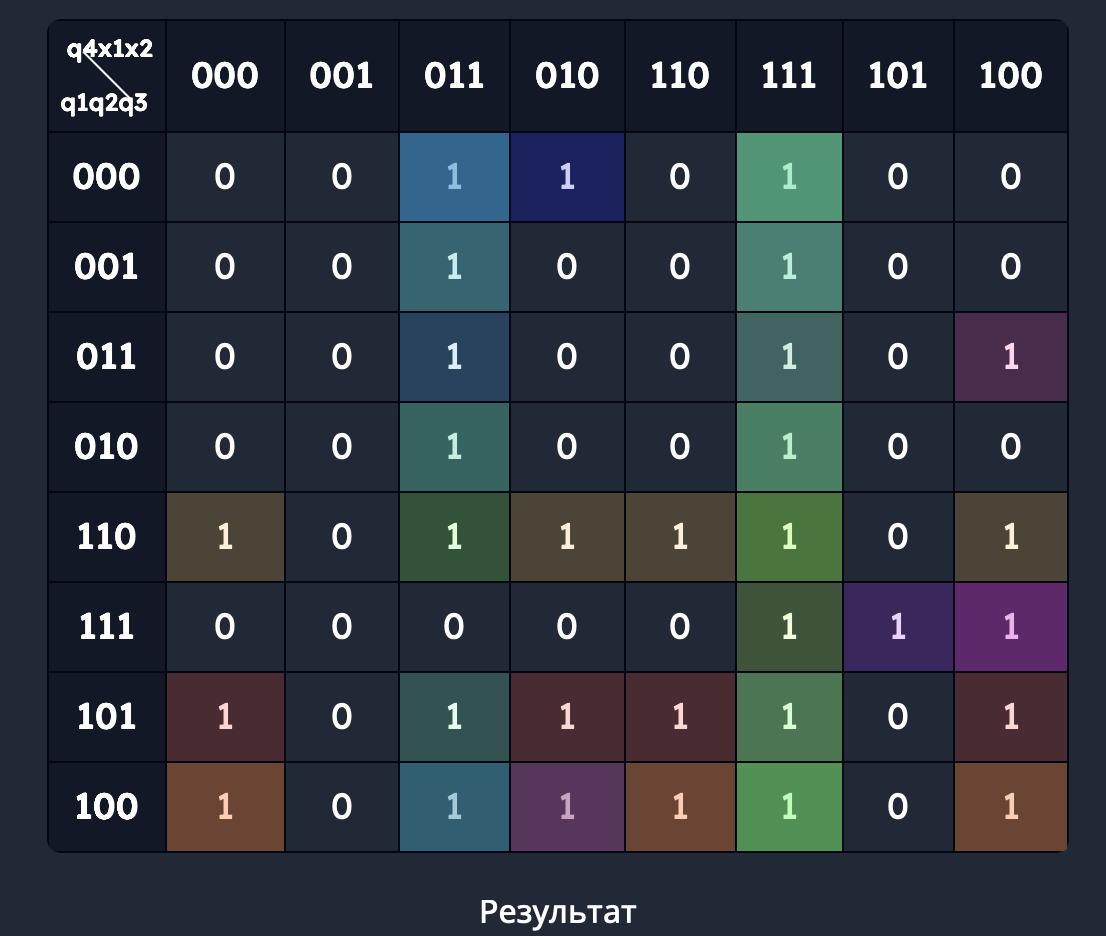
\includegraphics[width=\linewidth]{img/Q1.png}
			\[
			F = q_1 \overline{q_2} \overline{x_2} \lor q_1 \overline{q_3} \overline{x_2} \lor q_4 x_1 x_2 \lor \overline{q_3} x_1 x_2 \lor \overline{q_2} x_1 x_2 \lor 
			\\ \lor q_1 x_1 x_2 \lor q_2 \overline{q_3} q_4 x_1 \lor q_1 q_2 q_3 q_4 x_1 \lor q_2 q_3 q_4 x_1 x_2
			\]
		\end{minipage}%
		\begin{minipage}{0.5\linewidth}
			\centering
			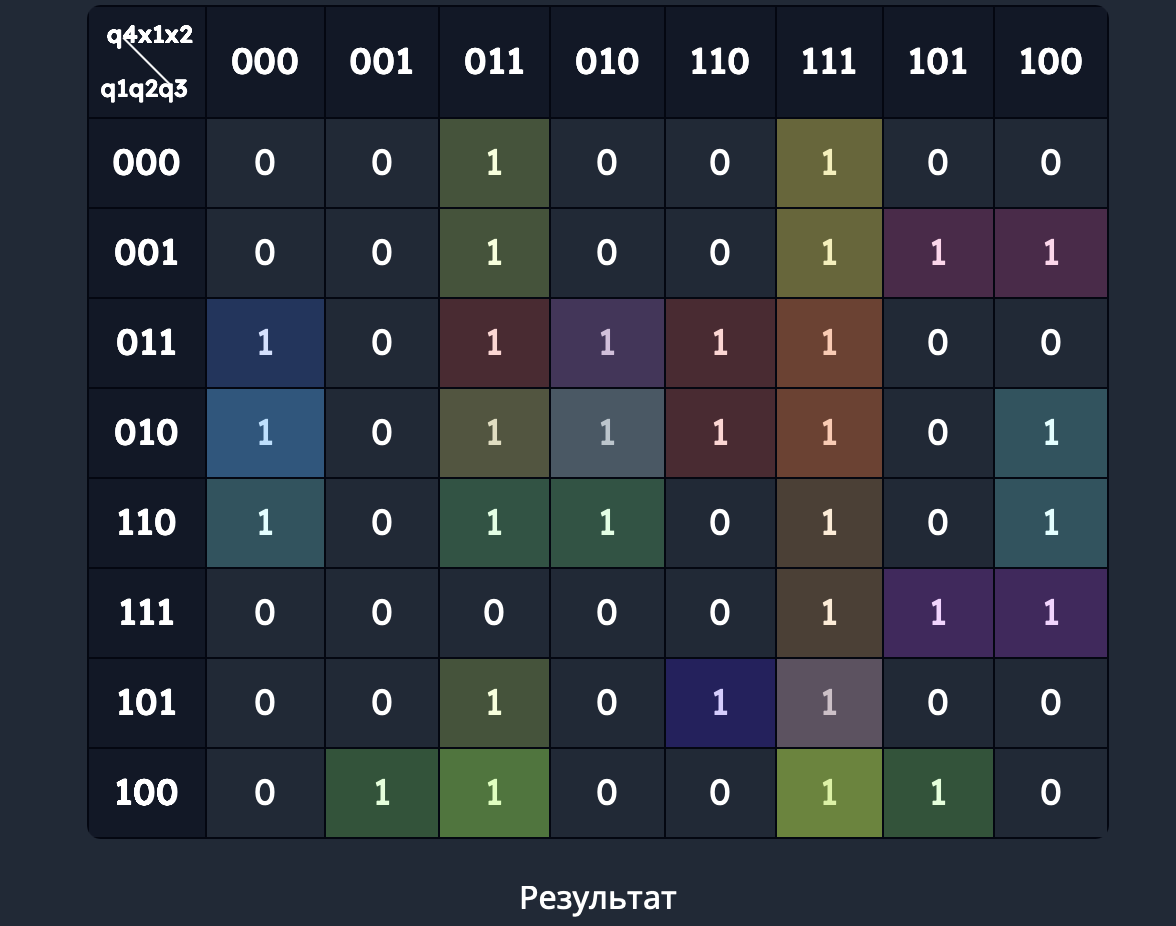
\includegraphics[width=\linewidth]{img/Q2.png}
			\[
			F = \overline{q_1} q_2 x_1 \lor q_4 x_1 x_2 \lor \overline{q_2} x_1 x_2 \lor q_1 \overline{q_2} q_3 x_2 \lor q_2 \overline{q_3} q_4 x_1 \lor 
			\\ \lor q_2 \overline{q_3} x_1 x_2 \lor q_1 q_2 q_4 x_2 \lor q_1 q_2 q_3 q_4 x_1 \lor q_1 q_2 q_3 q_4 x_1
			\]
		\end{minipage}
		\captionsetup{labelformat=empty}
		\caption{\hspace{1cm} Рис. 2: Минимизация Q1 \hspace{3cm} Рис. 3: Минимизация Q2}
		\label{Q:2}
	\end{figure}
	\setcounter{figure}{4}
	
	\vspace{0cm}\begin{figure}[h!]
		\vspace{0cm}\hspace{0cm}
		\begin{minipage}{0.5\linewidth}
			\centering
			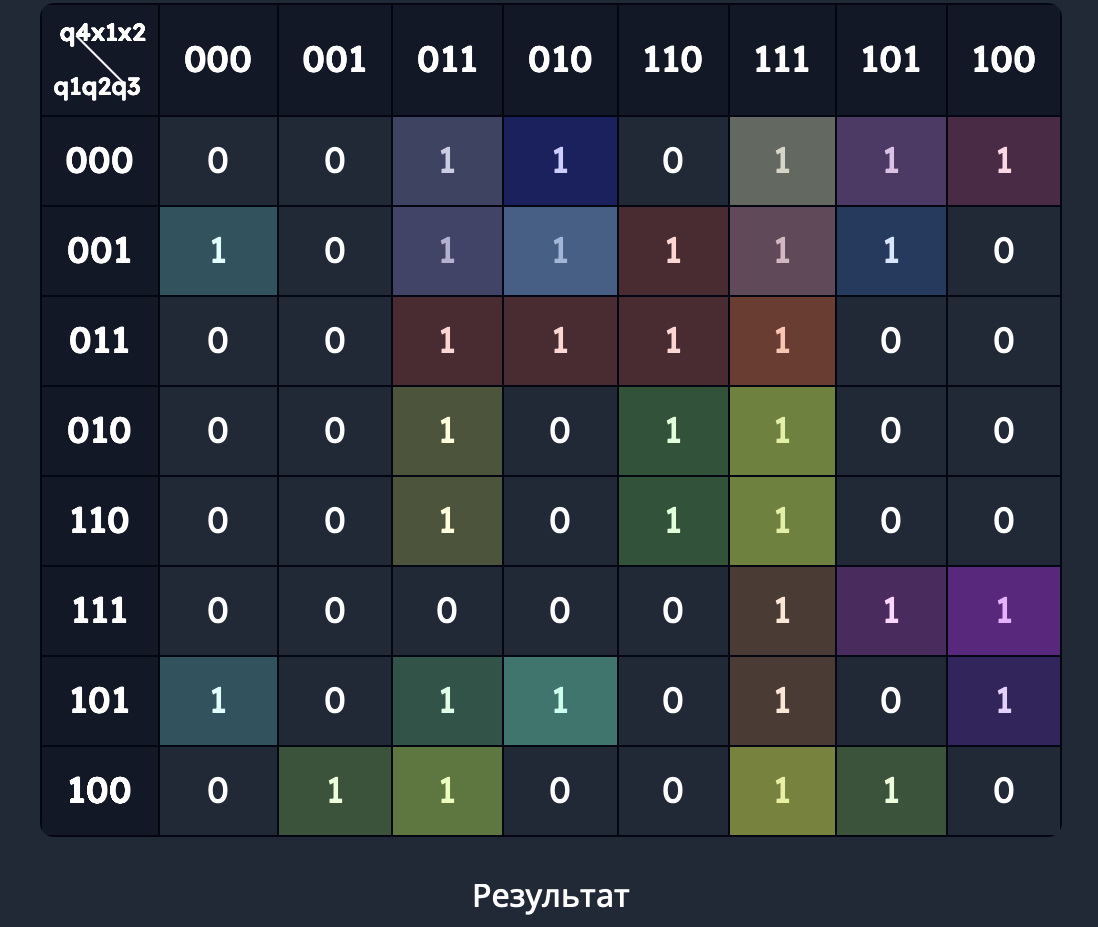
\includegraphics[width=\linewidth]{img/Q3.png}
			\[
			F = q_1 q_3 x_1 \lor q_4 x_1 x_2 \lor q_5 x_1 x_2 \lor q_1 q_2 q_3 x_2 \lor q_2 q_3 q_4 x_1 \lor 
			\\ \lor  q_2 q_3 q_4 x_1 \lor q_2 q_3 q_4 x_2 \lor q_1 q_2 q_4 x_2 \lor q_1 q_2 q_4 x_1 \lor \lor  q_1 q_3 q_4 x_1 x_2 \lor q_1 q_2 q_3 q_4 x_1 \lor q_1 q_2 q_3 q_4 x_1
			\]
		\end{minipage}%
		\begin{minipage}{0.5\linewidth}
			\centering
			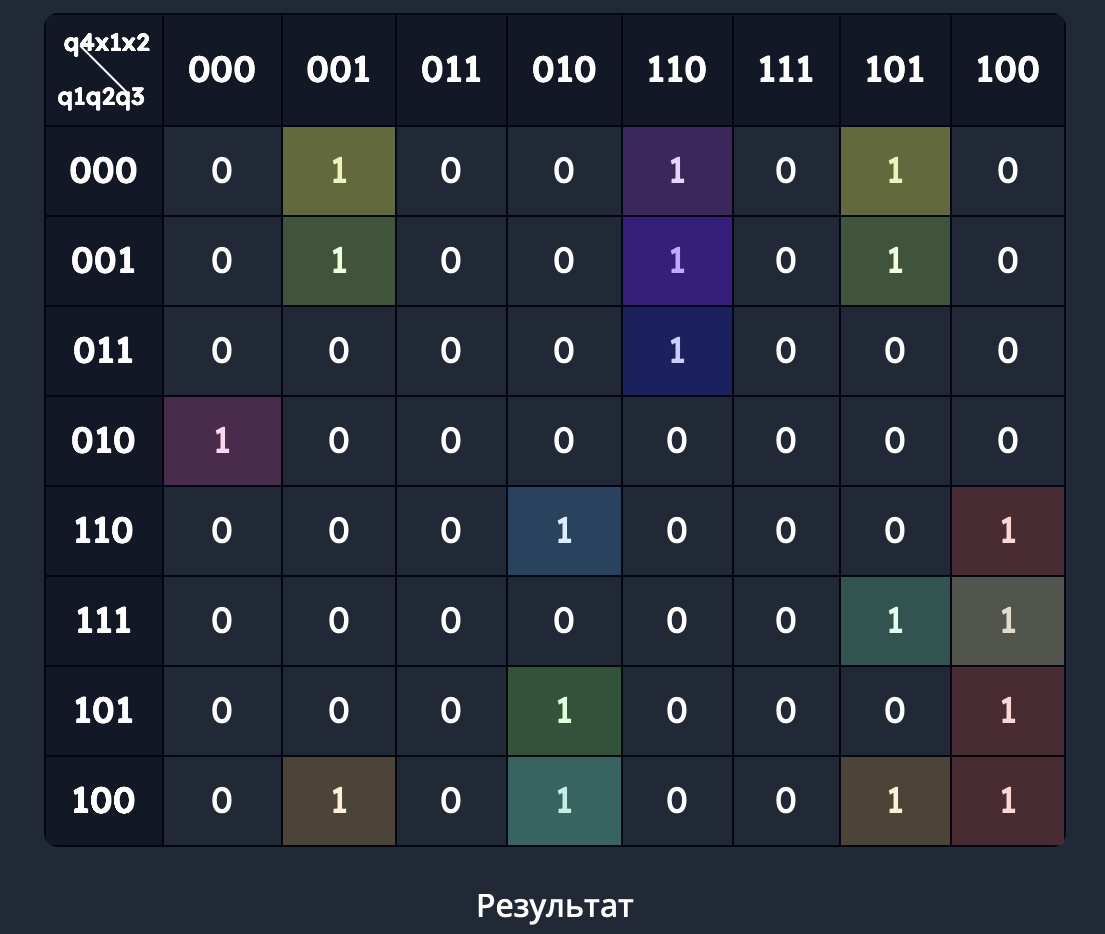
\includegraphics[width=\linewidth]{img/Q4.png}
			\[
			F = q_1 q_4 x_1 x_2 \lor q_2 q_3 x_1 x_2 \lor q_1 q_2 x_1 x_2 \lor q_1 q_2 q_4 x_1 x_2 \lor 
			\\  \lor q_1 q_2 q_3 q_4 x_1 \lor q_1 q_3 q_4 x_1 x_2 \lor q_1 q_2 q_4 x_1 x_2 \lor q_1 q_2 q_3 q_4 x_1 x_2
			\]
		\end{minipage}
		\captionsetup{labelformat=empty}
		\caption{\hspace{1cm} Рис. 4: Минимизация Q3 \hspace{3cm} Рис. 5: Минимизация Q4}
		\label{Q:5}
	\end{figure}
	\setcounter{figure}{5}
	
	Минимизация позволила сократить сложность логических выражений для каждого бита следующего состояния. Полученные функции используются для построения схемы, вычисляющей новое состояние автомата.
	
	
	\newpage
	\subsection{Минимизация L}
	
	На рисунках \ref{L:1}-\ref{L:8} изображена минимизация потециальных управляющих сигналов $L_1-L_8$ состояний конечного автомата при помощи Карт Карно.
	
	\vspace{0cm}\begin{figure}[h!]
		\vspace{0cm}\hspace{0cm}
		\begin{minipage}{0.45\linewidth}
			\centering
			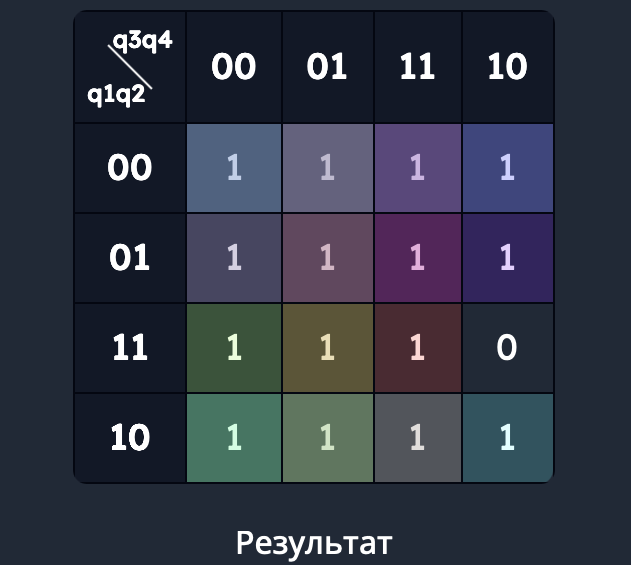
\includegraphics[width=\linewidth]{img/L1.png}
			\[ L_1 = q_4 \lor \overline{q_1} \lor \overline{q_2} \lor \overline{q_3} \]
		\end{minipage}
		\begin{minipage}{0.45\linewidth}
			\centering
			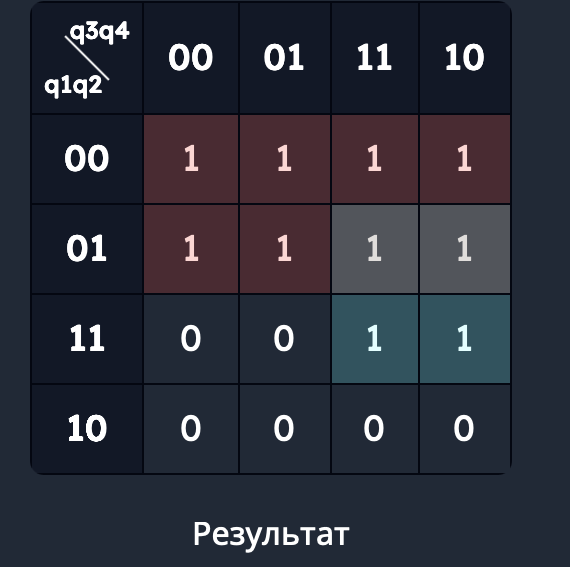
\includegraphics[width=\linewidth]{img/L2.png}
			\[ L_2 = \overline{q_1} \lor {q_2}{q_3}  \]
		\end{minipage}
		\captionsetup{labelformat=empty}
		\caption{Рис. 6: Минимизация L1 \hspace{2cm} Рис. 7: Минимизация L2}
		\label{L:1}
	\end{figure}
	
	\vspace{0cm}\begin{figure}[h!]
		\vspace{0cm}\hspace{0cm}
		\begin{minipage}{0.45\linewidth}
			\centering
			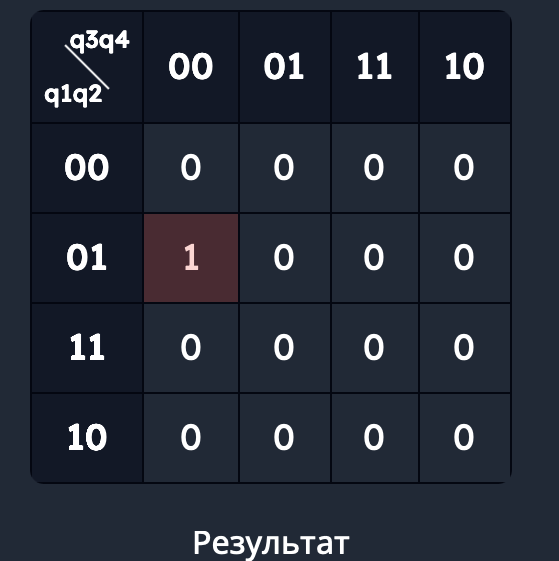
\includegraphics[width=\linewidth]{img/L3.png}
			\[ L_3 = \overline{q_1}{q_2}\overline{q_3}\overline{q_4} \]
		\end{minipage}
		\begin{minipage}{0.45\linewidth}
			\centering
			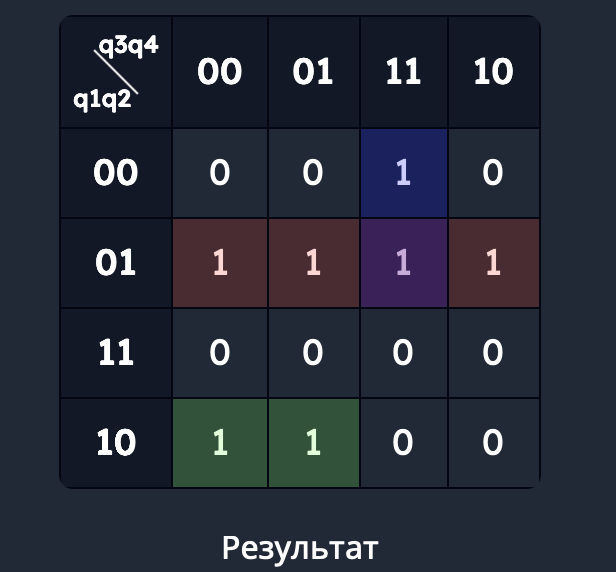
\includegraphics[width=\linewidth]{img/L4.png}
			\[ L_4 = \overline{q_1}{q_2} \lor  {q_1}\overline{q_2}\overline{q_3} \lor \overline{q_1}{q_3}{q_4} \]
		\end{minipage}
		\captionsetup{labelformat=empty}
		\caption{Рис. 8: Минимизация L3 \hspace{2cm} Рис. 9: Минимизация L4}
		\label{L:4}
	\end{figure}
	
	\vspace{0cm}\begin{figure}[h!]
		\vspace{0cm}\hspace{0cm}
		\begin{minipage}{0.45\linewidth}
			\centering
			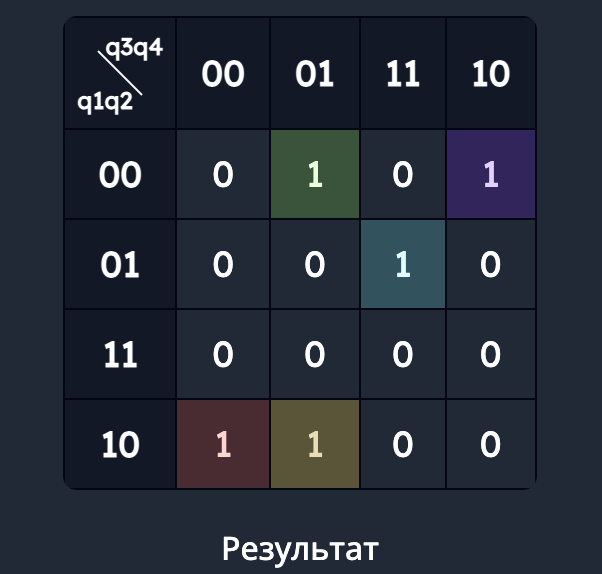
\includegraphics[width=\linewidth]{img/L5.png}
			\[ L_5 = {q_1}\overline{q_2}\overline{q_3} \lor \overline{q_2}\overline{q_3}{q_4} \lor \overline{q_1}{q_2}{q_3}{q_4} \lor \overline{q_1}\overline{q_2}{q_3}\overline{q_4}\]
		\end{minipage}
		\begin{minipage}{0.45\linewidth}
			\centering
			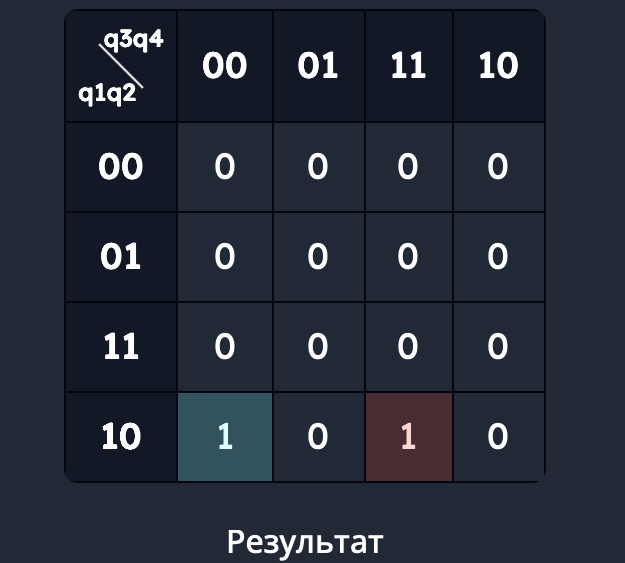
\includegraphics[width=\linewidth]{img/L6.png}
			\[ L_6 = {q_1}\overline{q_2}{q_3}{q_4} \lor {q_1}\overline{q_2}\overline{q_3}\overline{q_4} \]
		\end{minipage}
		\captionsetup{labelformat=empty}
		\caption{Рис. 10: Минимизация L5 \hspace{2cm} Рис. 11: Минимизация L6}
		\label{L:5}
	\end{figure}
	\setcounter{figure}{12}
	
	\vspace{0cm}\begin{figure}[h!]
		\vspace{0cm}\hspace{0cm}
		\begin{minipage}{0.45\linewidth}
			\centering
			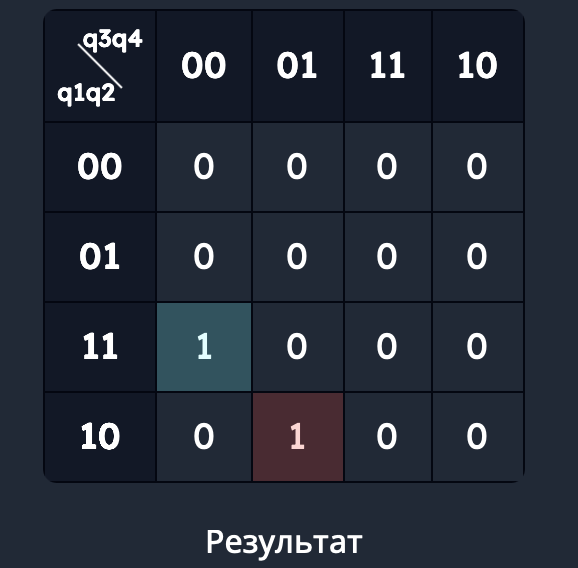
\includegraphics[width=\linewidth]{img/L7.png}
			\[ L_7 = {q_1}\overline{q_2}\overline{q_3}{q_4} \lor {q_1}{q_2}\overline{q_3}\overline{q_4} \]
		\end{minipage}
		\begin{minipage}{0.45\linewidth}
			\centering
			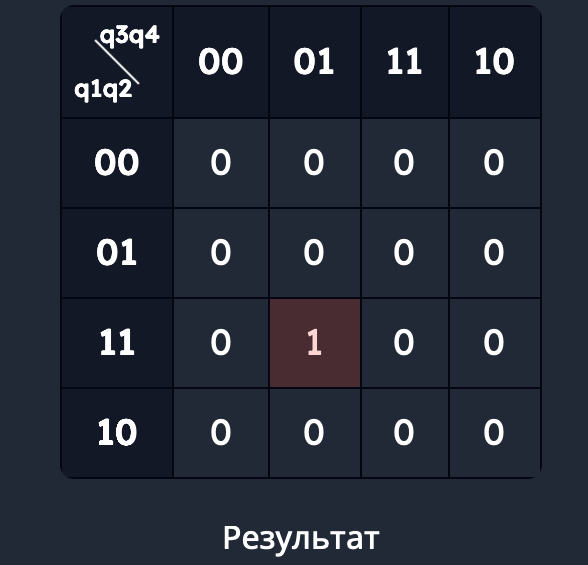
\includegraphics[width=\linewidth]{img/L8.png}
			\[ L_8 = {q_1}{q_2}\overline{q_3}{q_4} \]
		\end{minipage}
		\captionsetup{labelformat=empty}
		\caption{Рис. 12: Минимизация L7 \hspace{2cm} Рис. 13: Минимизация L8}
		\label{L:8}
	\end{figure}
	\setcounter{figure}{13}
	
	\needspace{5\baselineskip}{Каждая функция анализировалась отдельно, что позволило существенно сократить логические выражения. Например, \(L_1\) оказалась инверсной только к одному состоянию S14, \(L_3\) и \(L_8\) — простейшими конъюнкциями, а селекторные сигналы \(L_4, L_5\) свелись к комбинациям двух-трёх термов. Полученные минимальные формы минимизируют количество логических элементов при аппаратной реализации блока FL.}
	
	\newpage
	\subsection{Минимизация i}
	
	На рисунках \ref{i:1}-\ref{i:6} изображена минимизация импульсных управляющих сигналов $i_1-i_6$ состояний конечного автомата при помощи Карт Карно.
	\vspace{0cm}\begin{figure}[h!]
		\vspace{0cm}\hspace{0cm} 
		\begin{minipage}{0.32\linewidth}
			\centering
			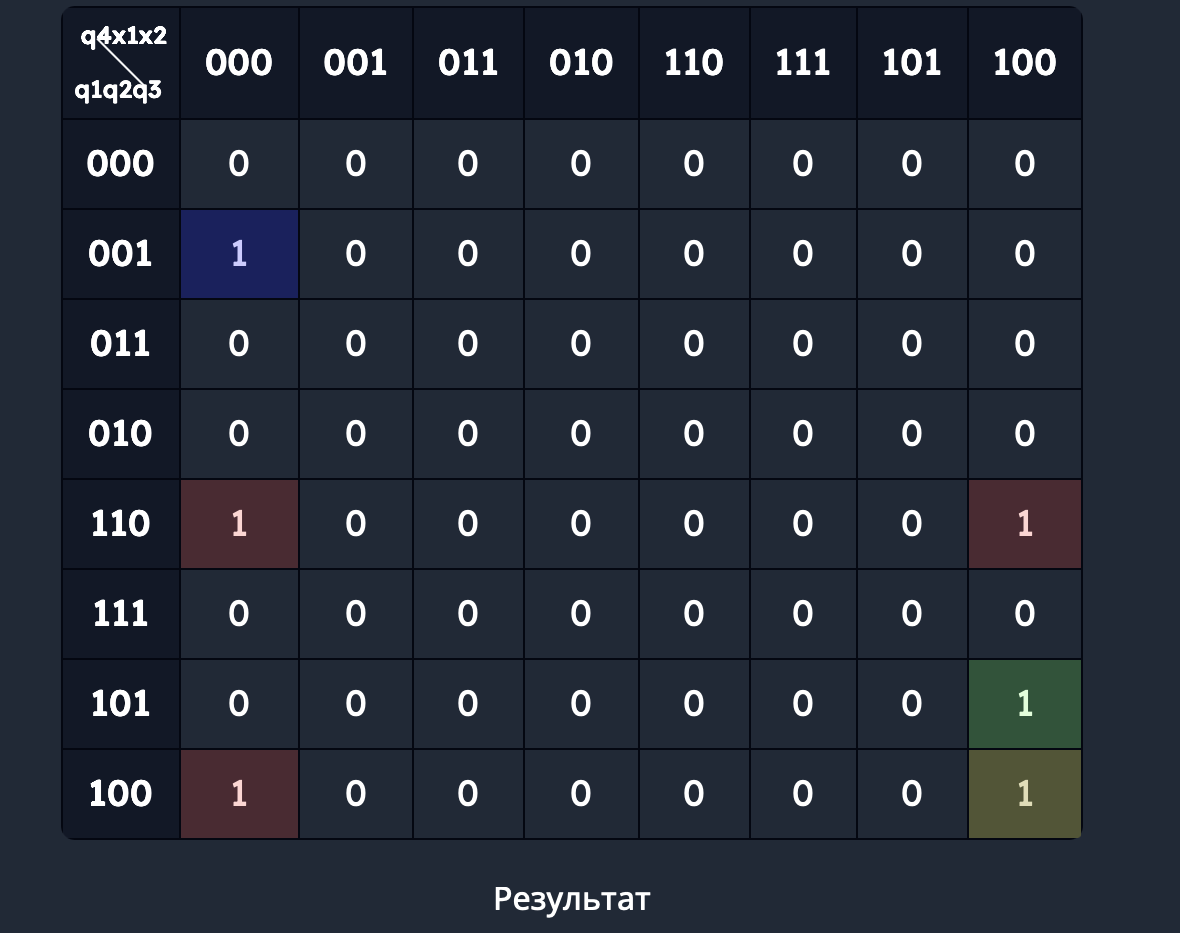
\includegraphics[width=\linewidth]{img/i1.png}
			\[ i_1 = {q_1}\overline{q_3}\overline{x_1}\overline{x_2} \lor {q_1}\overline{q_2}{q_4}\overline{x_1}\overline{x_2} \lor
			\\
			\lor  \overline{q_1}\overline{q_2}{q_3}\overline{q_4}\overline{x_1}\overline{x_2}\]
		\end{minipage}
		\begin{minipage}{0.32\linewidth}
			\centering
			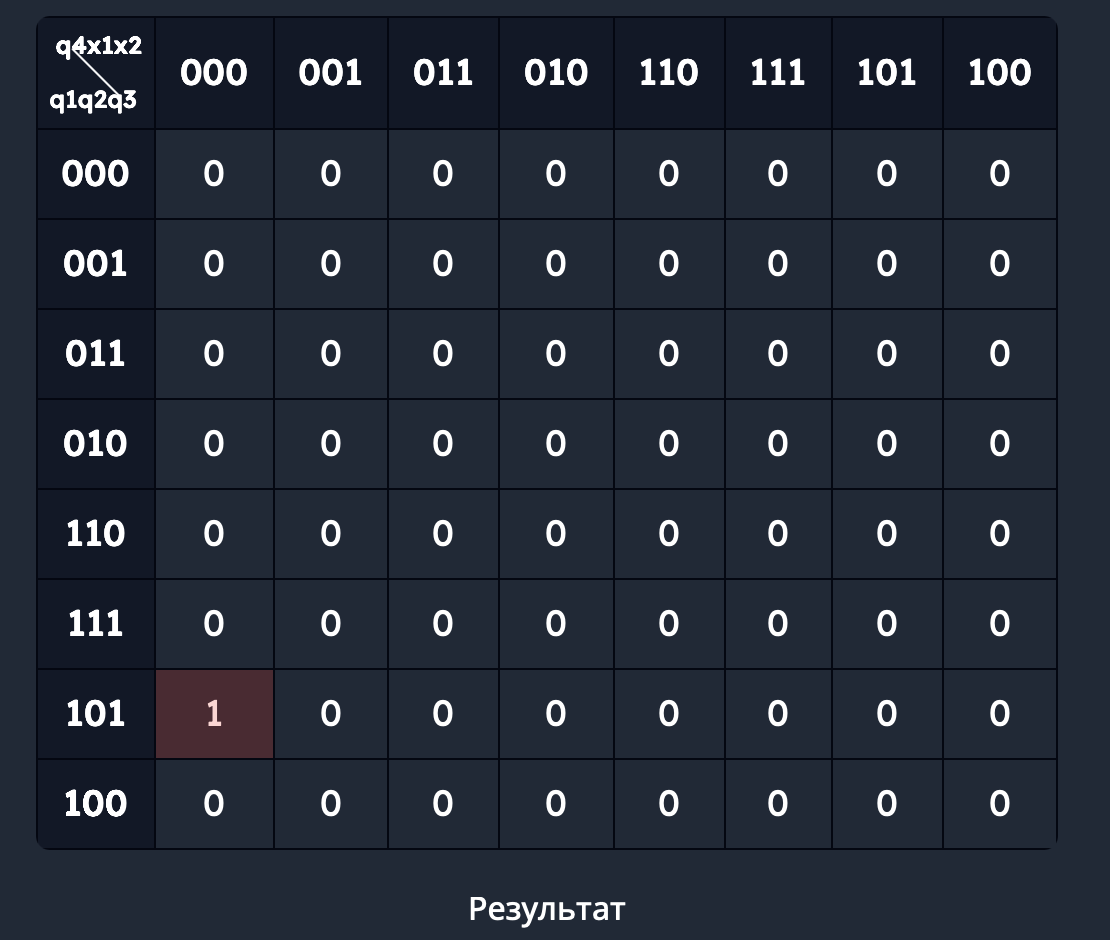
\includegraphics[width=\linewidth]{img/i2.png}
			\[ i_2 = q_1\overline{q_2}{q_3}\overline{q_4}\overline{x_1}\overline{x_2} \]
		\end{minipage}
		\begin{minipage}{0.32\linewidth}
			\centering
			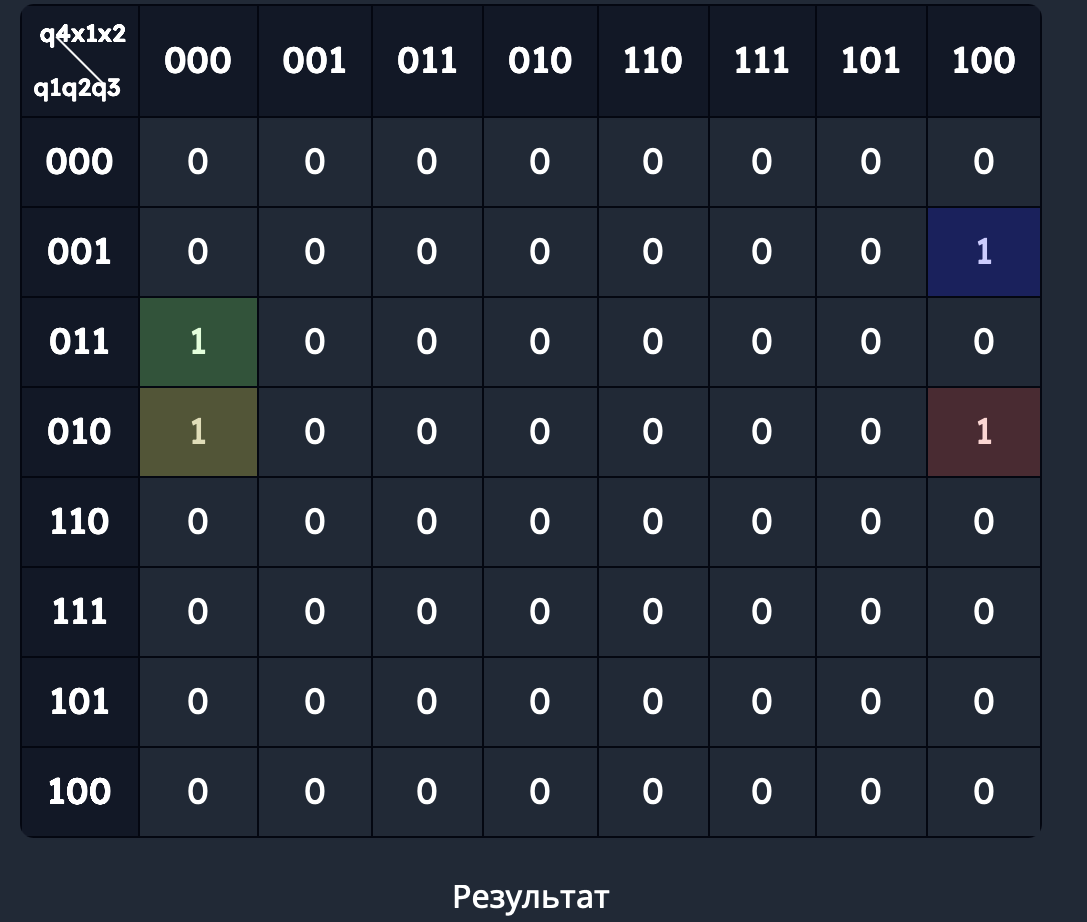
\includegraphics[width=\linewidth]{img/i3.png}
			\[ i_3 = \overline{q_1}{q_2}\overline{q_3}\overline{x_1}\overline{x_2} \lor \overline{q_1}{q_2}\overline{q_4}\overline{x_1}\overline{x_2} \lor
			\\
			\lor  \overline{q_1}\overline{q_2}{q_3}{q_4}\overline{x_1}\overline{x_2}\]
		\end{minipage}
		\captionsetup{labelformat=empty}
		\caption{Рис. 14: Минимизация i1 \hspace{1cm} Рис. 15: Минимизация i2 \hspace{1cm} Рис. 16: Минимизация i3}
		\label{i:1}
	\end{figure}
	\setcounter{figure}{18}
	
	\vspace{0cm}\begin{figure}[h!]
		\vspace{0cm}\hspace{0cm}
		\begin{minipage}{0.32\linewidth}
			\centering
			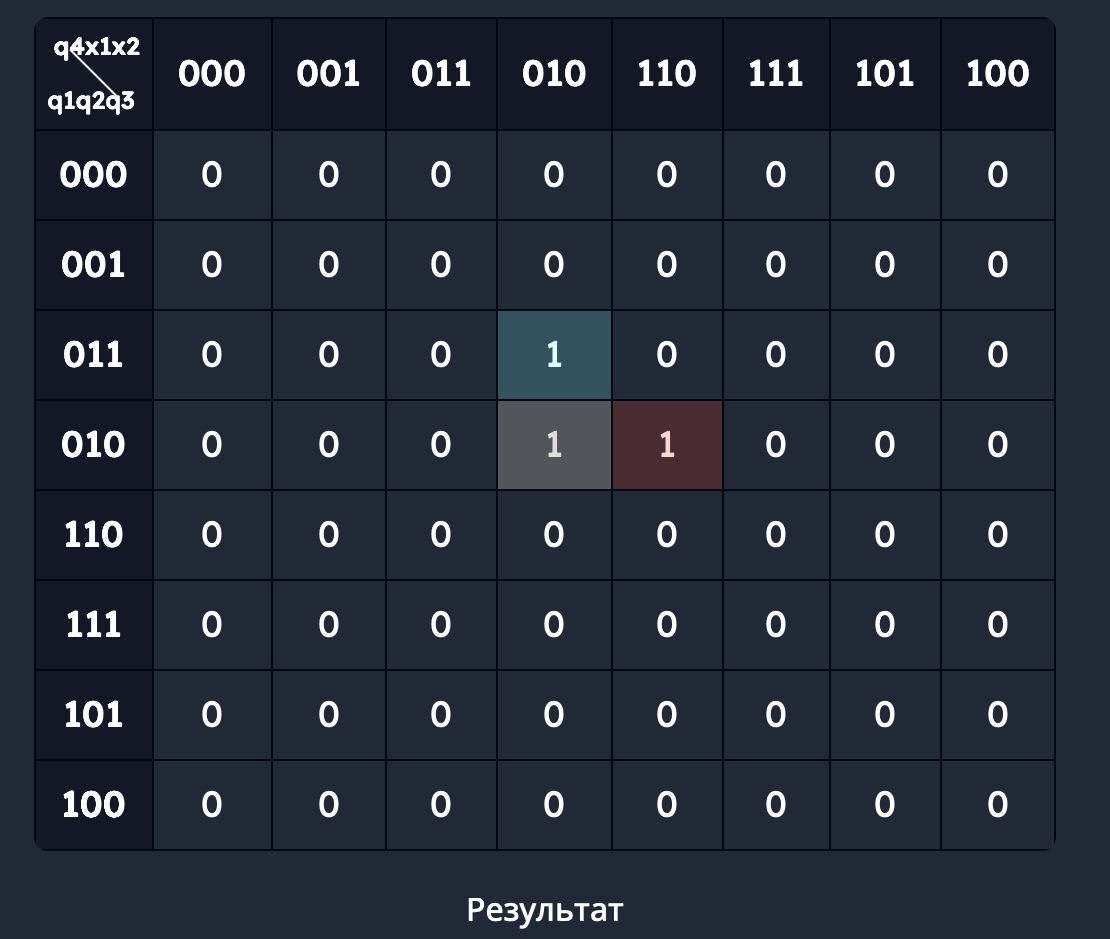
\includegraphics[width=\linewidth]{img/i4.png}
			\[ i_4 = \overline{q_1}{q_2}\overline{q_3}{x_1}\overline{x_2} \land \overline{q_1}{q_2}\overline{q_4}{x_1}\overline{x_2}\]
		\end{minipage}
		\begin{minipage}{0.32\linewidth}
			\centering
			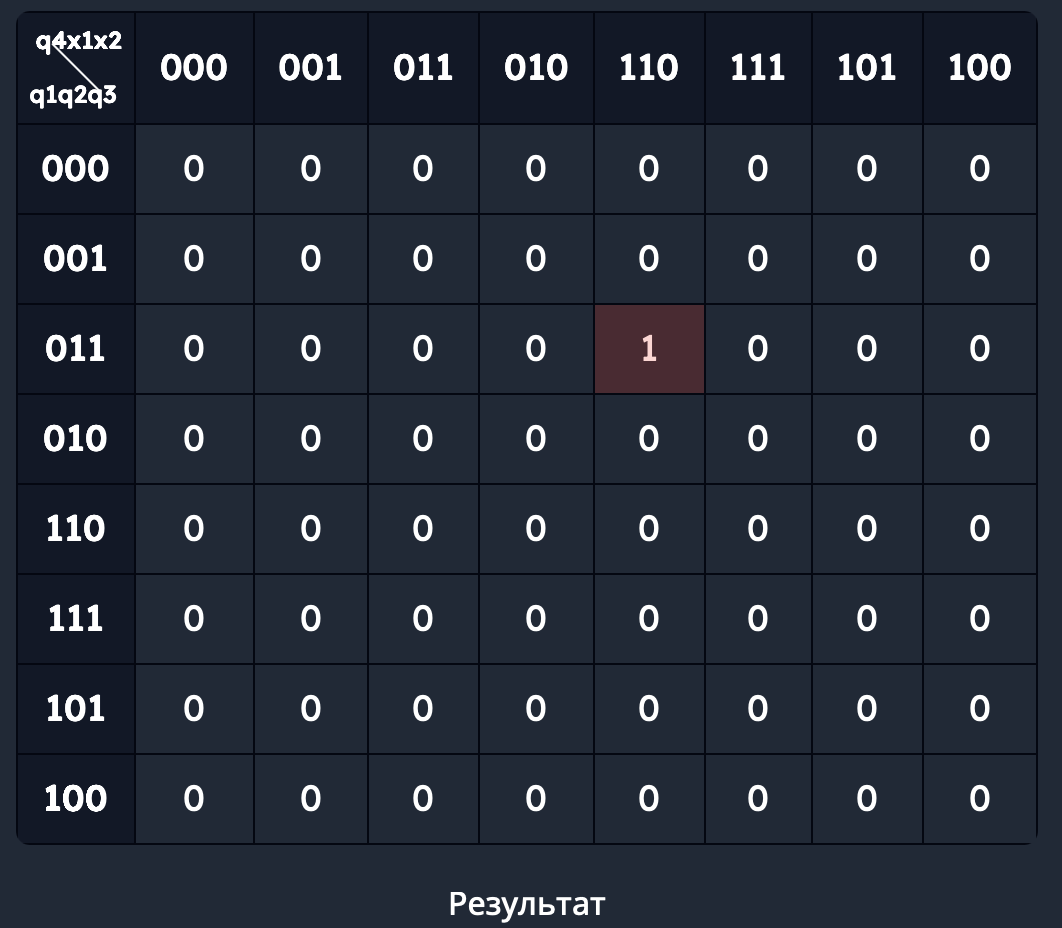
\includegraphics[width=\linewidth]{img/i5.png}
			\[ i_5 = \overline{q_1}{q_2}{q_3}{q_4}{x_1}\overline{x_2} \]
		\end{minipage}
		\begin{minipage}{0.32\linewidth}
			\centering
			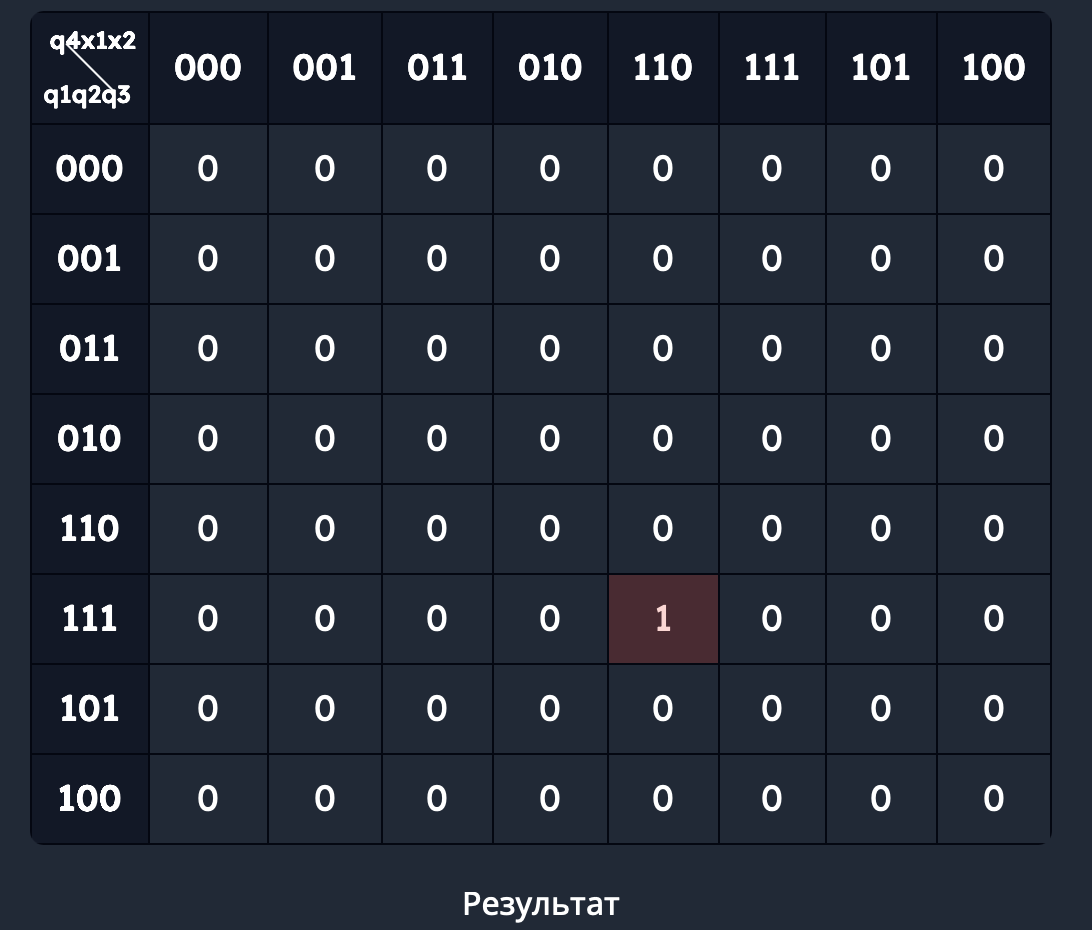
\includegraphics[width=\linewidth]{img/i6.png}
			\[ i_6 = {q_1}{q_2}{q_3}{q_4}{x_1}\overline{x_2} \]
		\end{minipage}
		\captionsetup{labelformat=empty}
		\caption{Рис. 17: Минимизация i4 \hspace{1cm} Рис. 18: Минимизация i5 \hspace{1cm} Рис. 19: Минимизация i6}
		\label{i:6}
	\end{figure}
	\setcounter{figure}{19}
	
	Каждая функция сведена к минимальной дизъюнктивной форме, что значительно упрощает аппаратную реализацию блока F. Полученные формулы обеспечивают корректное формирование управляющих импульсов при нажатиях кнопок в соответствующих состояниях автомата.
		
	\newpage
	\section{Схемотехническая реализация}
	\subsection{Индикаторный преобразователь}
	Для отображения чисел используются  индикаторы, содержащие семь сегментов, которые, высвечиваясь в определенной комбинации, могут 
	дать изображение цифры (см. рисунок \hyperref[indicator]{20}).  Для того чтобы сегмент “загорелся”, на него необходимо подать напряжение. Один разряд индикатора, таким образом, содержит 7 входов. Если на некоторые из этих входов подадим напряжение, а на остальные – нет, то на индикаторе высветится соответствующая комбинация сегментов. Например рисунок \hyperref[digit2]{(21)}, для изображения цифры <<2>> необходимо подать напряжение на все сегменты, кроме f1 и f4. 
	
	Функциональный преобразователь, который по двоичному 
	коду десятичной цифры вырабатывает сигналы, управляющие индикаторами называется индикаторный преобразователь (ИП). Его условное изображение дано на рисунке \hyperref[IC]{22}. 
	
	\begin{figure}[htpb]
		\centering
		\begin{minipage}{0.45\textwidth}
			\centering
			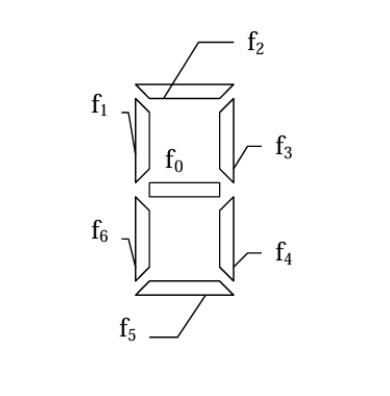
\includegraphics[scale=0.8]{img/1.png}
			\caption{Семисегментный индикатор}
			\label{indicator}
		\end{minipage}
		\hfill
		\begin{minipage}{0.45\textwidth}
			\centering
			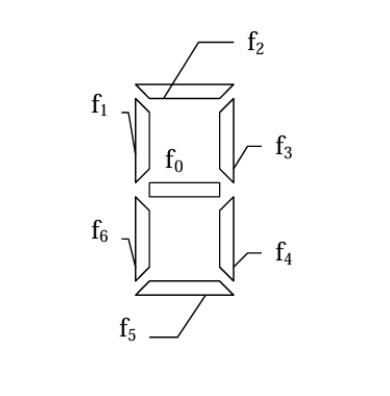
\includegraphics[scale=0.8]{img/1.png}
			\caption{Изображение цифры <<2>>}
			\label{digit2}
		\end{minipage}
		\hfill
		\begin{minipage}{0.9\textwidth}
			\centering
			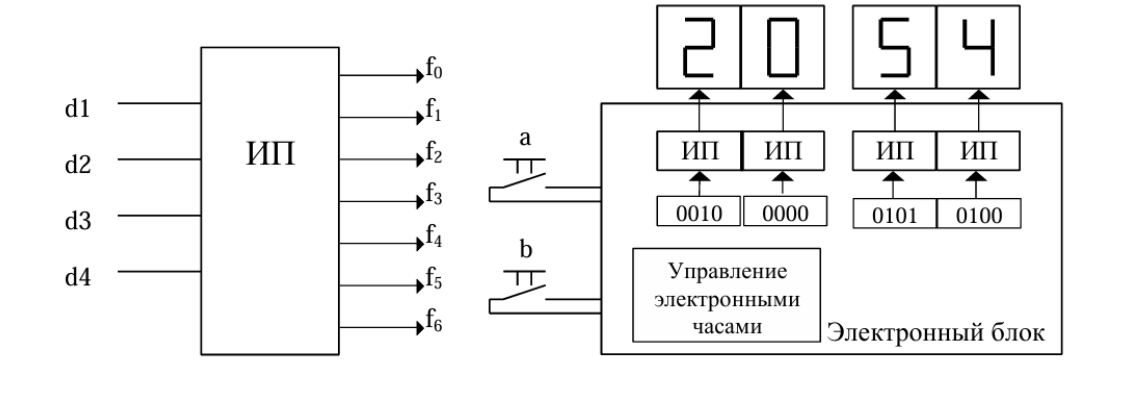
\includegraphics[scale=0.8]{img/3.png}
			\caption{Индикаторный преобразователь}
			\label{IC}
		\end{minipage} 
	\end{figure}
	
	Схема индикаторного преобразователя представлена на рисунке \hyperref[IC_ready]{23}.
	
	\begin{figure}[htpb]
		\centering
		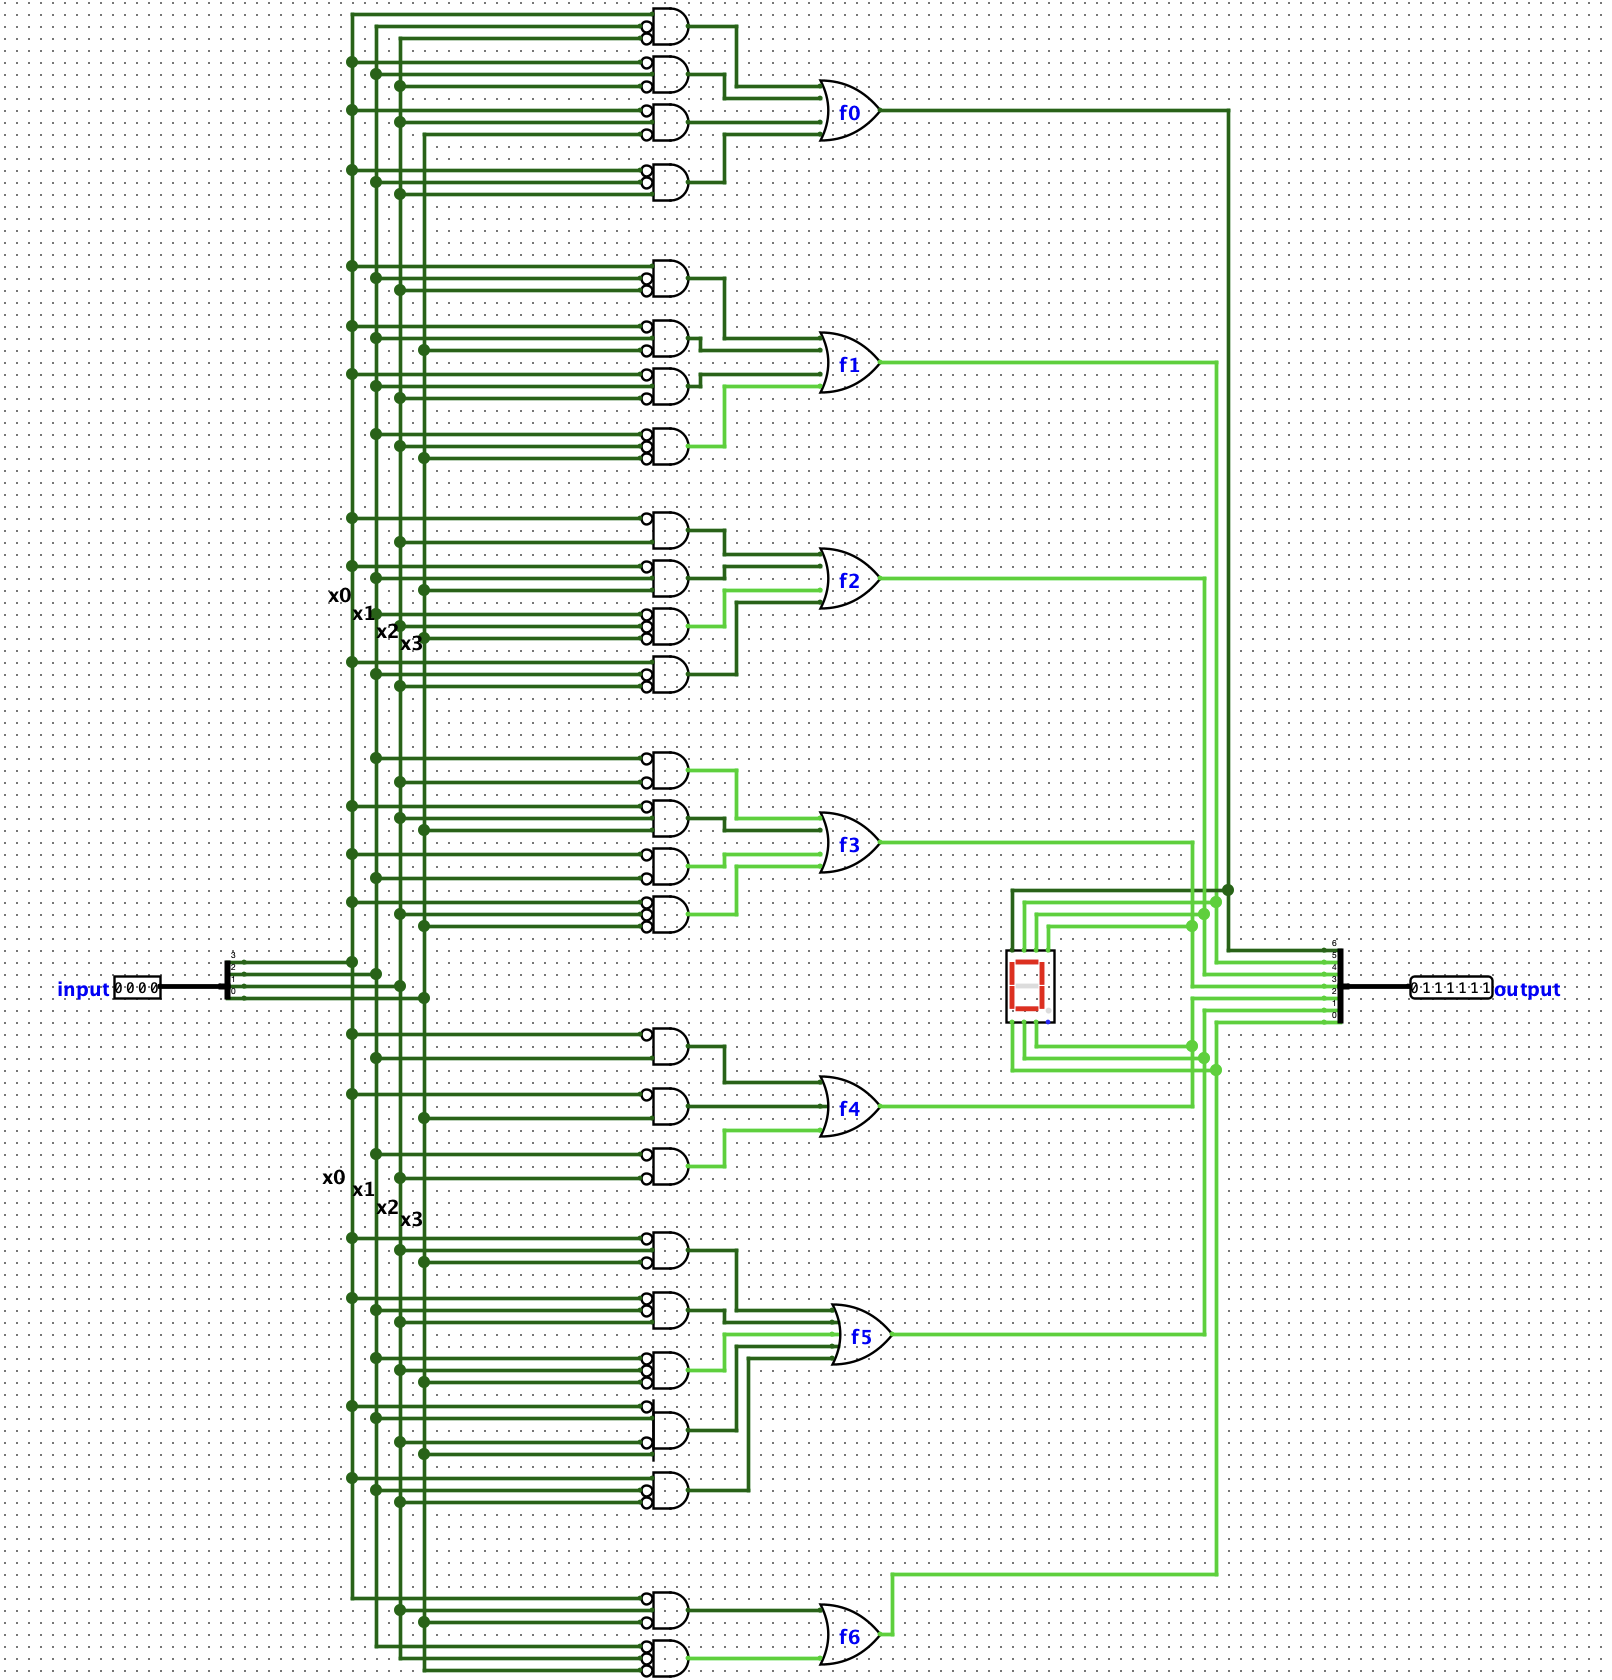
\includegraphics[scale=0.6]{img/4.png}
		\label{IC_ready} 
		\caption{Схема индикаторного преобразователя}
	\end{figure}
	
	\newpage
	
	\textbf{Тактовый генератор}
	
	Тактовый генератор (или генератор тактовых импульсов) — это электронное устройство, которое создает периодические электрические импульсы (такты), используемые для синхронизации работы различных компонентов электронных устройств. 
	
	В электронных часах применяют малогабаритные стабильные генераторы, с выхода которых снимается последовательность прямоугольных импульсов. Частота кварцевых генераторов стабильна, она практически не изменяется во времени.
	
	\begin{figure}[htpb]
		\centering
		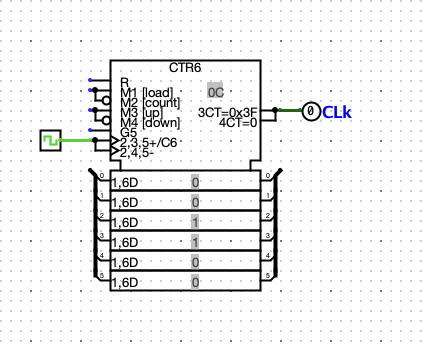
\includegraphics[scale=0.6]{img/16.png}
		\label{tact} 
		\caption{Схема индикаторного преобразователя}
	\end{figure}
	
	Для получения частоты 1 Гц используется делитель частоты (счетчик), понижающий частоту системного генератора, пример показан на рисунке \hyperref[IC_ready]{24}.
	\subsection{Счетчик}
	
	Для реализации функции отсчета времени используются счетчики, управляемые генератором тактовых импульсов. 
	
	Счетчик - это устройство, которое осуществляет счет и хранение кода числа подсчитанных импульсов. У каждого счетчика есть тактовый вход, на который поступают электрические импульсы, и несколько выходов, с которых можно снимать двоичный код числа, находящийся в счетчике. С каждым новым входным импульсом этот код увеличивается на 1.
	
	Важным параметром счетчика является коэффициент пересчета К. К - это максимальное число импульсов, которое может быть подсчитано. Если рассматривать счетчик как конечный автомат, то К - это количество 
	различных состояний счетчика. Счетчик с коэффициентом пересчета К через К переключений возвращается в исходное состояние. Для удобства использования счетчика, кроме тактового входа существует вход <<Уст.0>> (сброс). При подаче на него импульса (логической единицы) на выходе устанавливается нулевой код.
	
	Пример счетчика для отчета секунд изображен на рисунке \hyperref[counters]{25}.
	
	\begin{figure}[htpb]
		\centering
		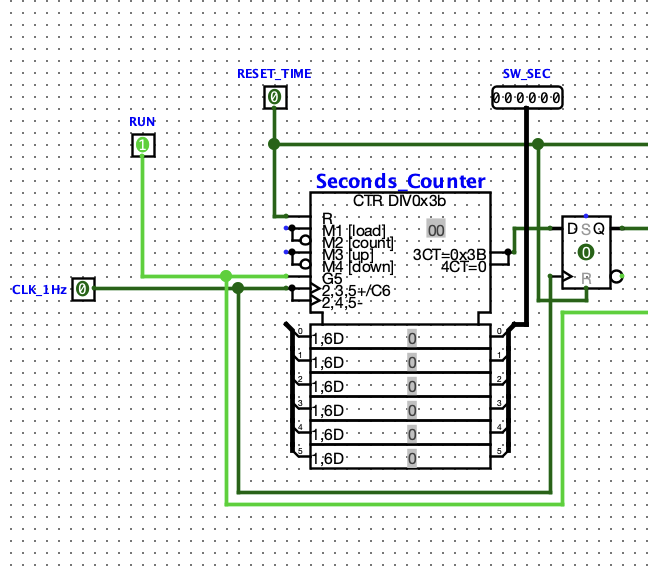
\includegraphics[scale=0.4]{img/5.png}
		\label{counters} 
		\caption{Схема счетчиков для отсчета секунд}
	\end{figure}
	
	\newpage
	\textbf{D-триггер}
	
	Триггер -- устройство с двумя устойчивыми состояниями. Основная его функция - хранить один бит информации неограниченное время до тех пор, пока эта информация не будет изменена воздействием на вход триггера. Существует довольно много разновидностей триггеров, различающихся по входным условиям смены состояния. 
	
	D-триггер имеет два основных входа:
	\begin{enumerate}
		\item D (Data) — данные, которые будут записаны в триггер.
		\item CLK (Clock) — тактовый сигнал, который управляет процессом записи.
	\end{enumerate}
	
	Также у него есть два выхода:
	\begin{enumerate}
		\item Q — выход, который отражает текущее состояние триггера (хранит данные).
		\item $\overline{\text{Q}}$ — инвертированное состояние выхода Q.
	\end{enumerate}
	
	
	Микросхема D-триггера изображена на рисунке \hyperref[D-trigger]{26}.
	
	\begin{figure}[htpb]
		\centering
		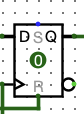
\includegraphics[scale=0.8]{img/6.png}
		\label{D-trigger} 
		\caption{Микросхема D-триггера}
	\end{figure}
	
	\textbf{T-триггер}
	
	Т-триггер (Toggle flip-flop) — это счетный триггер, который изменяет свое состояние на противоположное при каждом поступлении тактового импульса, если на счетном входе T (Toggle) присутствует логическая единица. Если на входе T логический ноль, состояние триггера не меняется.
	
	Логика работы описывается следующим уравнением:
	\[ Q(t+1) = Q(t) \oplus T \]
	
	В разработанной схеме Т-триггеры используются для реализации переключения режимов (например, включение/выключение будильника) и для хранения бита AM/PM, который должен инвертироваться при переходе через 12 часов.
	
	\begin{figure}[htpb]
		\centering
		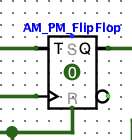
\includegraphics[scale=0.8]{img/30.png}
		\label{T-trigger} 
		\caption{Т-триггер}
	\end{figure}
	
	Условное графическое обозначение Т-триггера приведено на рисунке \hyperref[T-trigger]{27}.
	
	\subsection{Цифровой компаратор}
	Цифровой компаратор — это комбинационное логическое устройство, предназначенное для сравнения двух двоичных чисел (A и B) одинаковой разрядности.
	
	Компаратор имеет три выходных сигнала, которые указывают на результат сравнения:
	\begin{itemize}
		\item $A > B$ (A больше B)
		\item $A = B$ (A равно B)
		\item $A < B$ (A меньше B)
	\end{itemize}
	
	\begin{figure}[htpb]
		\centering
		% ЗАМЕНИТЬ ПУТЬ НА СВОЙ ФАЙЛ
		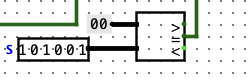
\includegraphics[scale=0.8]{img/31.png}
		\label{comparator} 
		\caption{Цифровой компаратор}
	\end{figure}
	
	В схеме часов компараторы широко используются для:
	\begin{itemize}
		\item Сравнения текущего времени с установленным временем будильника (для формирования сигнала звонка).
		\item Определения момента сброса счетчиков (например, при достижении 12 часов или 60 минут).
		\item Определения состояния автомата для управления индикацией.
	\end{itemize}
	
	Изображение компаратора приведено на рисунке \hyperref[comparator]{28}.
	
	\subsection{Постоянное запоминающее устройство (ПЗУ)}
	Постоянное запоминающее устройство (ПЗУ, англ. ROM — Read-Only Memory) — это энергонезависимая память, предназначенная для хранения неизменяемых данных. В контексте проектирования конечных автоматов и схем управления ПЗУ часто используется как таблица поиска (Look-Up Table, LUT) для реализации сложных логических функций.
	
	Принцип работы ПЗУ заключается в выдаче данных, хранящихся в ячейке памяти, адрес которой подается на адресный вход.
	
	В разработанной схеме часов ПЗУ применяется в блоке управления дисплеем (\textbf{DisplayMux}). На адресный вход ПЗУ подается код текущего состояния автомата (State), а с выхода считываются управляющие маски:
	\begin{itemize}
		\item Сигналы гашения неиспользуемых разрядов индикаторов (например, отключение отображения часов в режиме секундомера).
		\item Управляющие сигналы для выбора источника AM/PM (основное время, часовой пояс или будильник).
	\end{itemize}
	
	\begin{figure}[htpb]
		\centering
		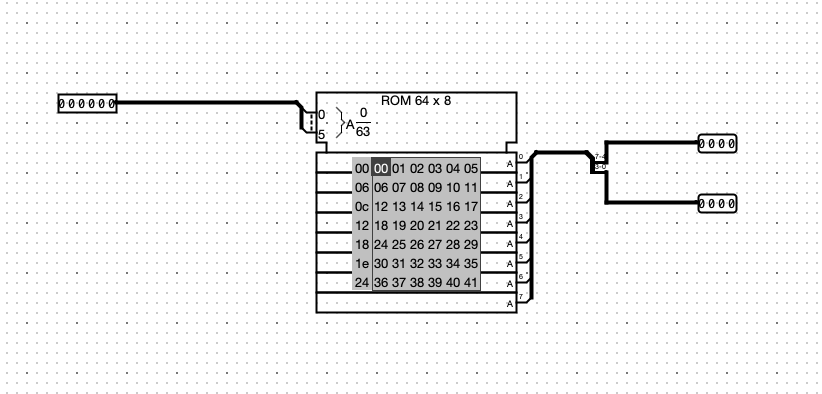
\includegraphics[scale=0.6]{img/22.png}
		\label{rom} 
		\caption{Постоянное запоминающее устройство (ROM)}
	\end{figure}
	
	Использование ПЗУ позволило существенно упростить схему дешифрации режимов отображения и избежать громоздкой комбинационной логики на логических элементах.
	
	Условное обозначение ПЗУ приведено на рисунке \hyperref[rom]{29}.
	
	
	\subsection{Мультиплексор}
	Мультиплексор (Mux) — это коммутационное устройство, которое передает сигнал с одного из нескольких информационных входов на один выход. Выбор конкретного входа осуществляется с помощью управляющих сигналов (селекторов).
		
	Функционально мультиплексор можно представить как управляемый переключатель. Если мультиплексор имеет $N$ адресных входов, то он может переключать $2^N$ информационных входов.
	
	
	\begin{figure}[htpb]
		\centering
		% ЗАМЕНИТЬ ПУТЬ НА СВОЙ ФАЙЛ
		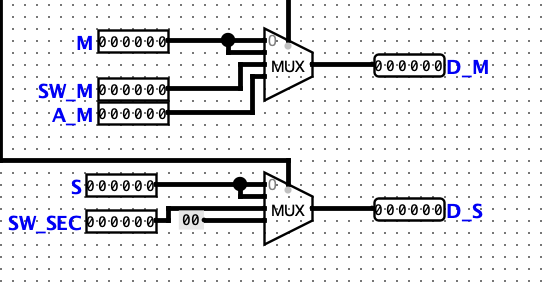
\includegraphics[scale=0.8]{img/32.png}
		\label{mux} 
		\caption{Мультиплексор}
	\end{figure}
	
	В данной работе мультиплексоры играют ключевую роль в блоке \textbf{DisplayMux}, обеспечивая переключение отображаемой информации на дисплее (текущее время / секундомер / настройки будильника) в зависимости от текущего состояния управляющего автомата.
	
	Условное обозначение мультиплексора показано на рисунке \hyperref[mux]{30}.
	
	\subsection{Преобразователь внешних воздействий}
	Данный блок предназначен для конвертации нажатой кнопки в соответствующие сигналы $x_0$ и $x_1$. Также он создает синхроимпульс, который необходим для работы в блоке памяти.
	Схема преобразователя внешних воздействий изображена на рисунке \hyperref[BC]{31}.
	\begin{figure}[htpb]
		\centering
		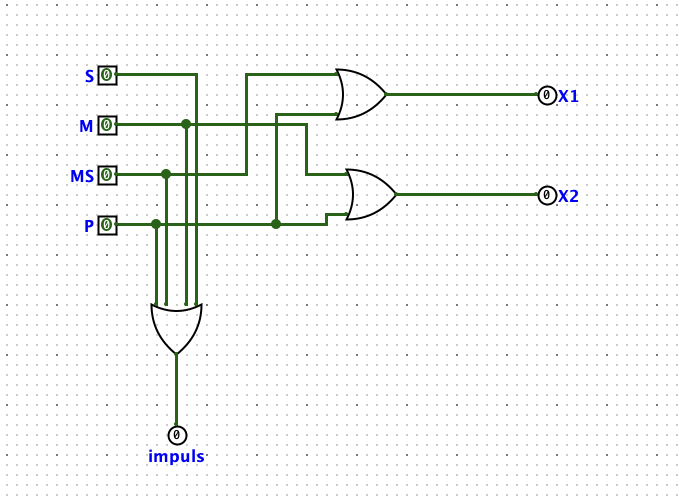
\includegraphics[scale=0.4]{img/10.png}
		\label{BC} 
		\caption{Схема преобразователя кнопок}
	\end{figure}
	
	\subsection{Блок F}
	Блок F предназначен для вычисления следующего состояния на основе текущего состояния и входных данных (кнопок). Помимо следующего состояния вычисляются  импульсные сигналы необходимы при переходе в следующее состояние.
	
	Схема блока F представлена на рисунке \hyperref[F0-block]{32}, а также представлены блоки Q1,Q2,Q3,Q4 на рисунках \hyperref[F1-block]{33 - 36}.
	
	\begin{figure}[htpb]
		\centering
		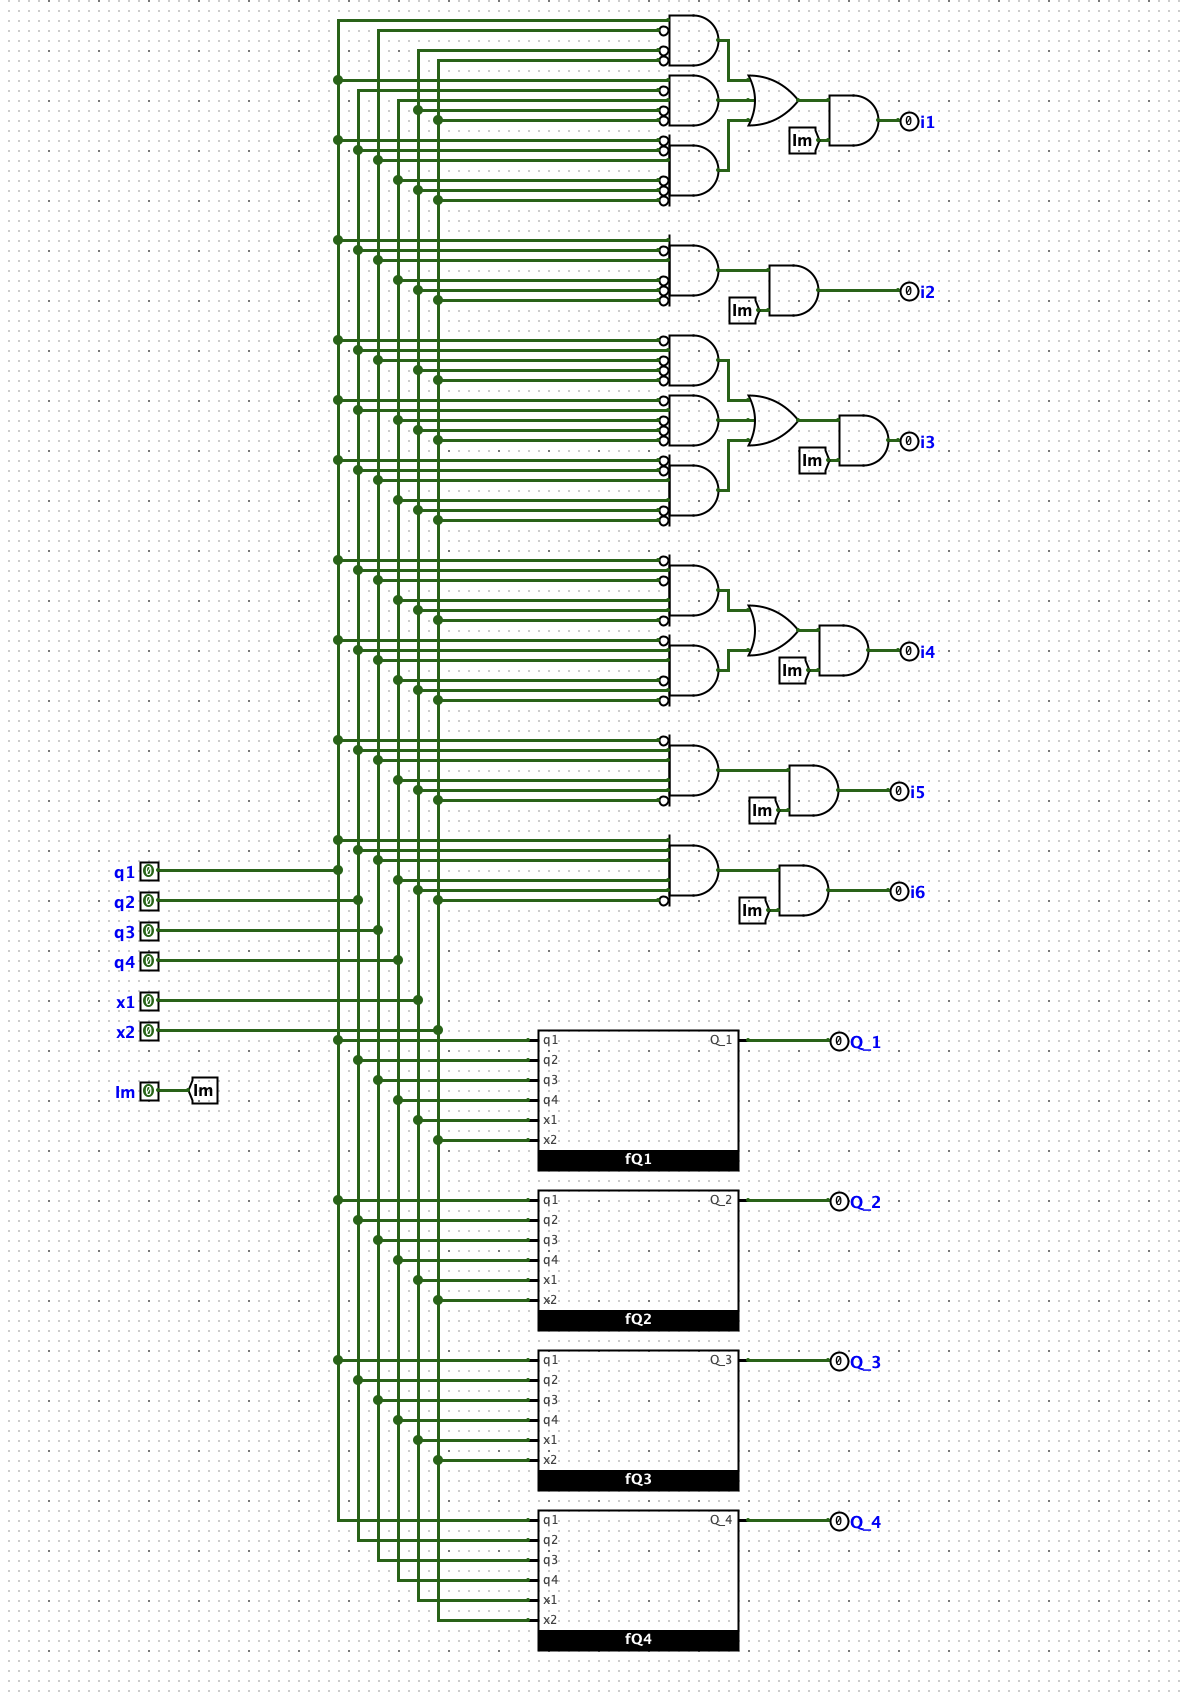
\includegraphics[scale=0.6]{img/7.png}
		\label{F0-block} 
		\caption{Схема блока F}
	\end{figure}
	
	\begin{figure}[htpb]
		\centering
		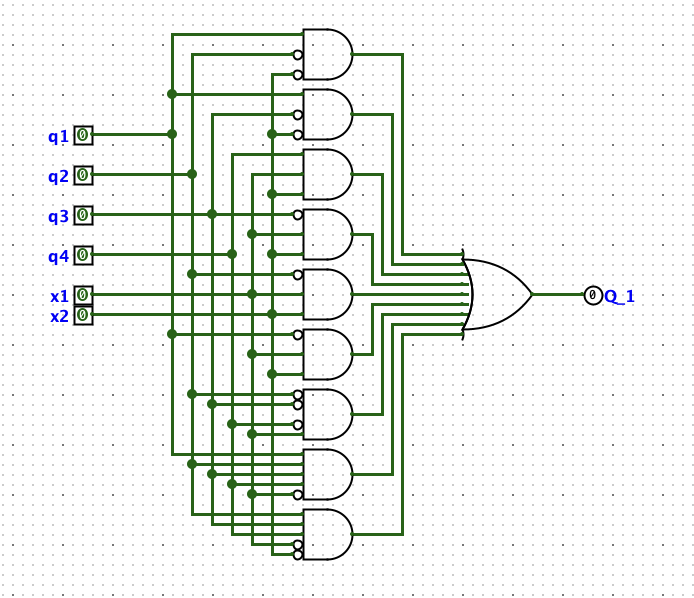
\includegraphics[scale=0.6]{img/17.png}
		\label{F1-block} 
		\caption{Схема блока Q1}
	\end{figure}
	
	
	\begin{figure}[htpb]
		\centering
		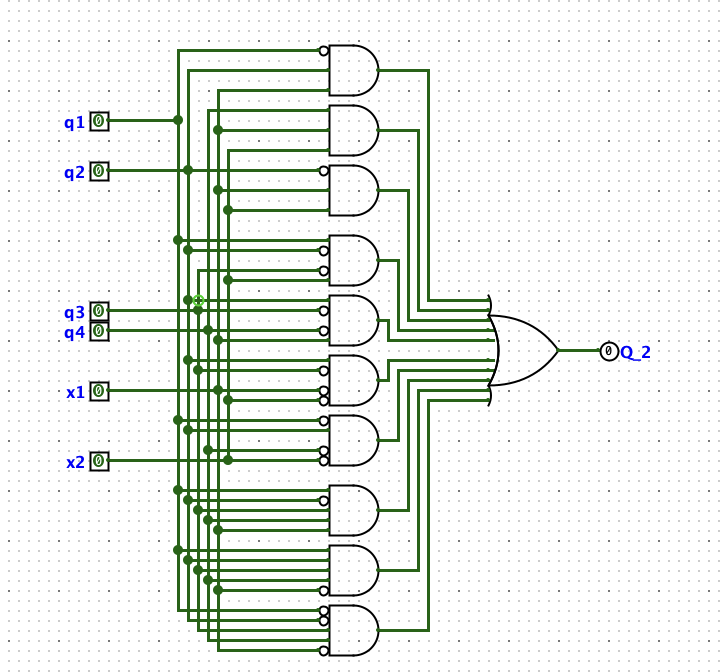
\includegraphics[scale=0.6]{img/18.png}
		\label{F-block} 
		\caption{Схема блока Q2}
	\end{figure}
	
	
	\begin{figure}[htpb]
		\centering
		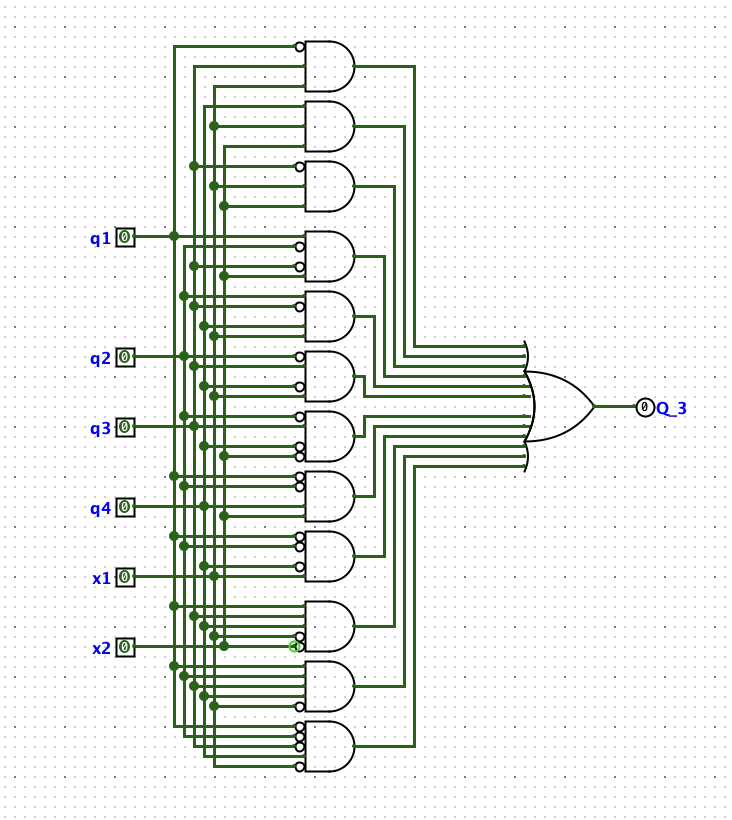
\includegraphics[scale=0.6]{img/19.png}
		\label{F-block} 
		\caption{Схема блока Q3}
	\end{figure}
	
	
	\begin{figure}[htpb]
		\centering
		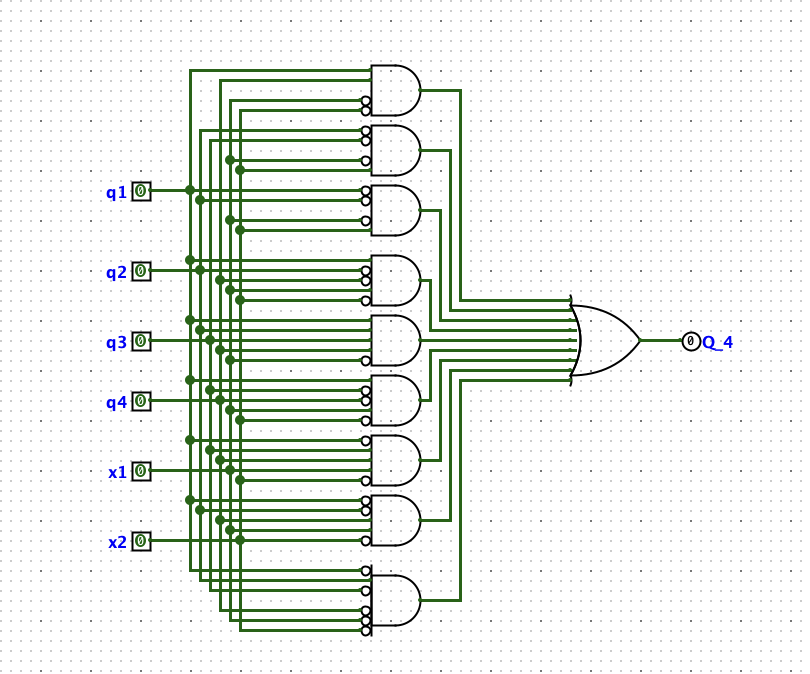
\includegraphics[scale=0.6]{img/20.png}
		\label{F-block} 
		\caption{Схема блока Q4}
	\end{figure}
	
	\newpage
	\subsection{Блок памяти}
	Блок памяти предназначен для хранения текущего состояния автомата. Схема блока памяти изображена на рисунке \hyperref[memory]{37}.
	\begin{figure}[htpb]
		\centering
		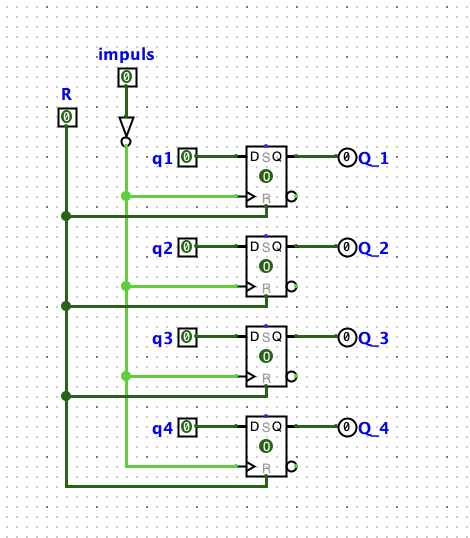
\includegraphics[scale=0.6]{img/8.png}
		\label{memory} 
		\caption{Схема блока памяти}
	\end{figure}
	
	
	
	\subsection{Блок FL}
	Блок FL отвечает за формирование потенциальных сигналов на основе  текущего состояния автомата. Схема блока FL представлена на рисунке \hyperref[FL-block]{38}.
	\begin{figure}[htpb]
		\centering
		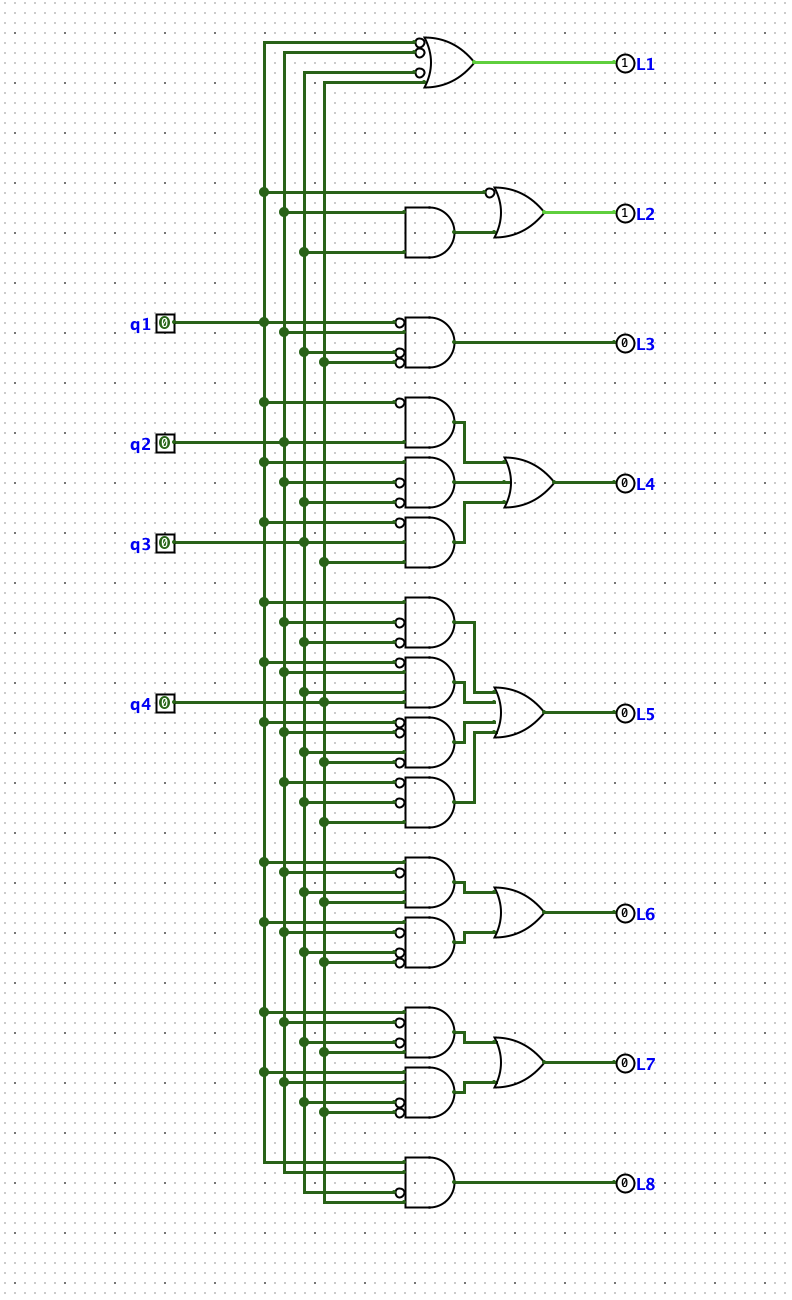
\includegraphics[scale=0.4]{img/9.png}
		\label{FL-block} 
		\caption{Схема блока FL}
	\end{figure}
	
	\subsection{Машина состояний}
	Данная схема представляет машину состояний или конечный автомат электронных часов. Она предназначена для переключения состояний в зависимости от входных сигналов. Она состоит из блоков F, FL и блока памяти.
	
	Схема конечного автомата часов представлена на рисунке \hyperref[state machine]{39}.
	\begin{figure}[htpb]
		\centering
		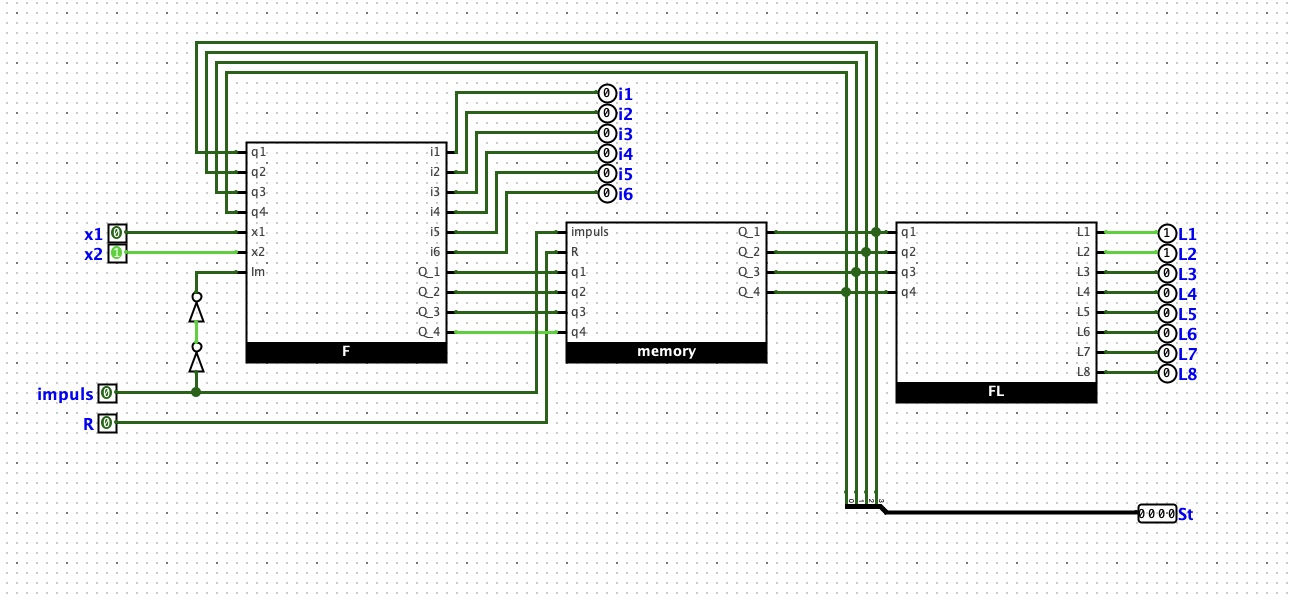
\includegraphics[scale=0.4]{img/11.png}
		\label{state machine} 
		\caption{Схема конечного автомата часов }
	\end{figure}
	
	
	\subsection{Отсчет времени часов}
	Данная схема предназначена для отсчета времени часов. Она состоит из системы счетчиков.  
	Схема отсчета времени у часов представлена на рисунке \hyperref[clock]{40}.
	\begin{figure}[htpb]
		\centering
		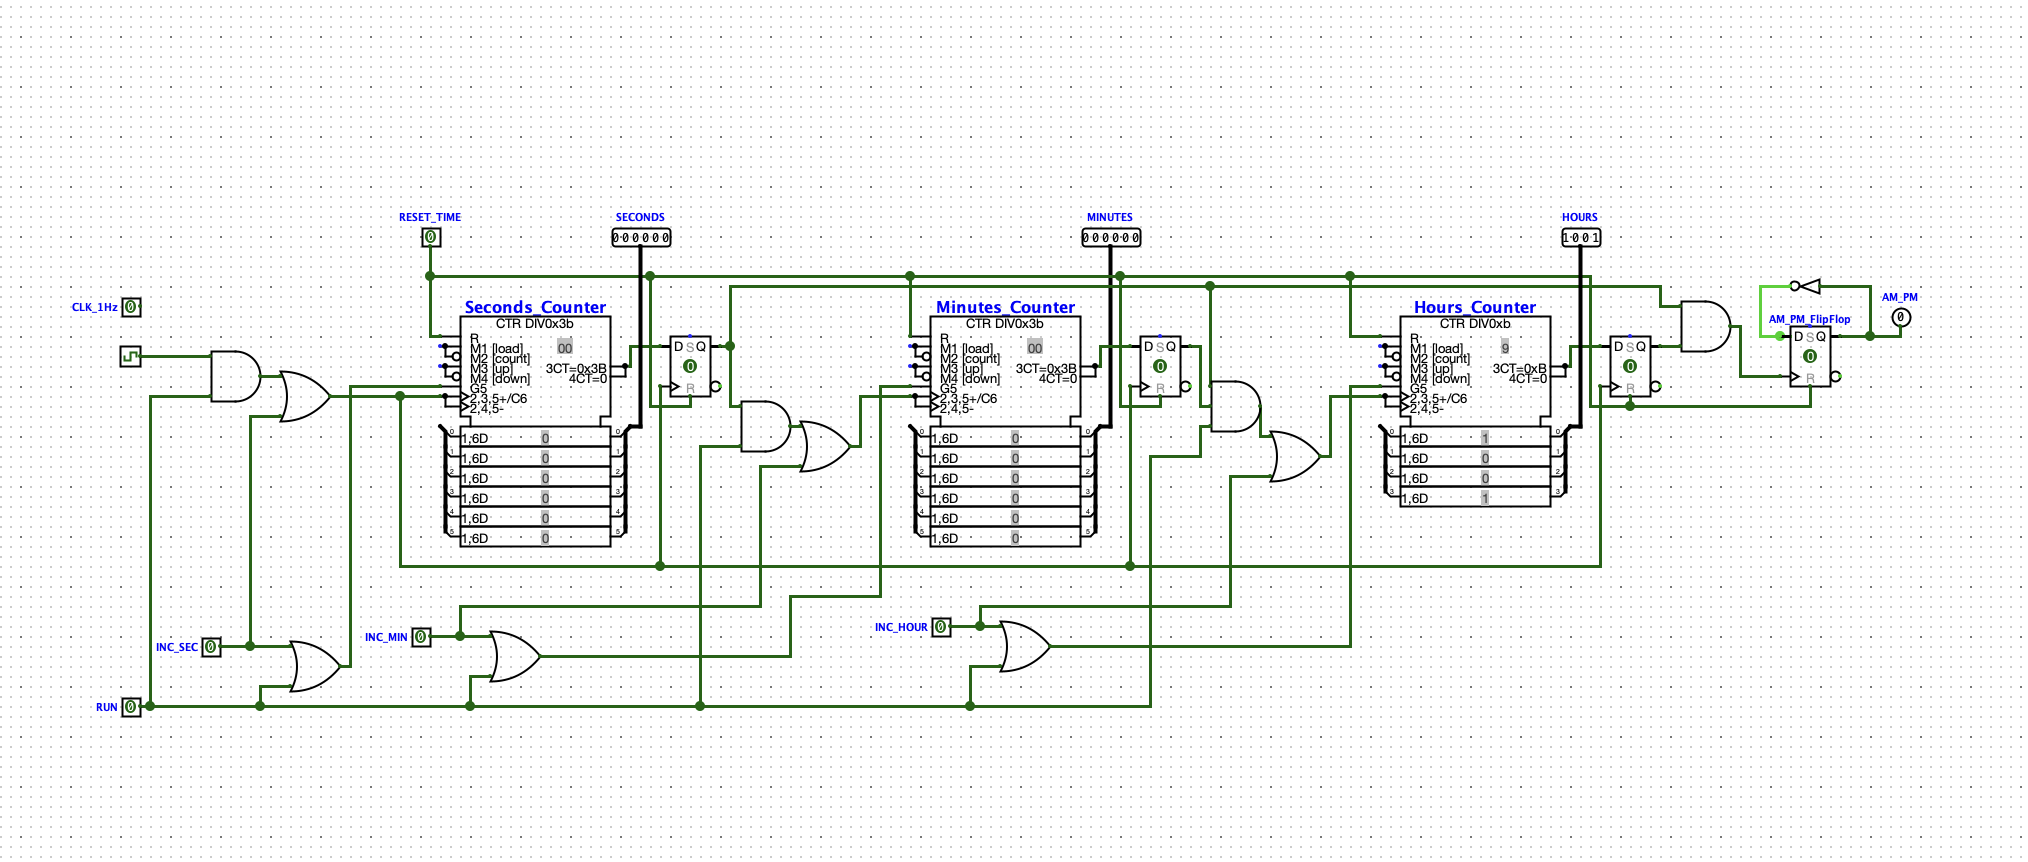
\includegraphics[scale=0.5]{img/12.png}
		\label{clock} 
		\caption{Схема отсчета времени часов }
	\end{figure}
	
	
	\subsection{Блоки SplitterHours и SplitterTime}
	Данные блоки предназначены для преобразования двоичного кода времени в четырех-битный для того, чтобы разбить контанты часов, минут, секунд на блоки десятков и едениц, пригодных для вывода на индикаторы(IndicatorConvector).
	\begin{itemize}
		\item \textbf{SplitterHours} — обрабатывает значение часов. Содержит логику для корректного отображения 12-часового формата (замена 0 на 12) рисунок  \hyperref[splitterH]{41}.
		\item \textbf{SplitterTime} — обрабатывает значения минут и секунд (диапазон 00-59) рисунок \hyperref[splitterM]{42}.
	\end{itemize}
	
	\begin{figure}[htpb]
		\centering
		% ЗАМЕНИТЬ ПУТЬ
		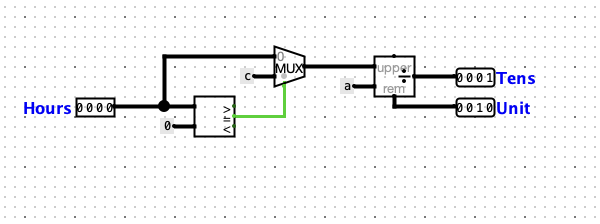
\includegraphics[scale=0.6]{img/23.png}
		\label{splitterH} 
		\caption{Схема блока SplitterHours}
	\end{figure}
	
		\begin{figure}[htpb]
		\centering
		% ЗАМЕНИТЬ ПУТЬ
		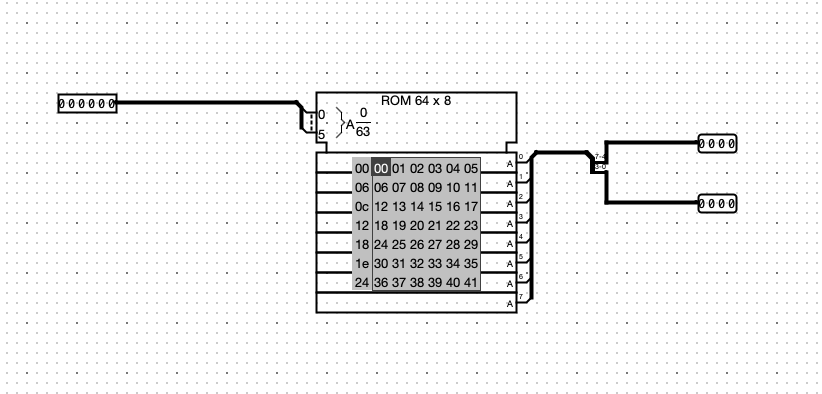
\includegraphics[scale=0.6]{img/22.png}
		\label{splitterM} 
		\caption{Схема блока SplitterTime}
	\end{figure}
	
	Схемы реализованы на базе комбинационной логики деления с остатком.

	
	\subsection{Decoder\_i1 (Формирователь импульсов)}
	Блок дешифрации управляющих сигналов. Его задача — преобразовать текущее состояние автомата и сигналы нажатия кнопок в конкретные импульсные микрокоманды (например, \(i\_m\) — инкремент минут, \(i\_h\) — инкремент часов, \(reset\) — сброс). Реализован на базе логических элементов И, сопоставляющих код состояния с входным воздействием, рисунок \hyperref[disp]{43}.
	
	\begin{figure}[htpb]
		\centering
		% ЗАМЕНИТЬ ПУТЬ
		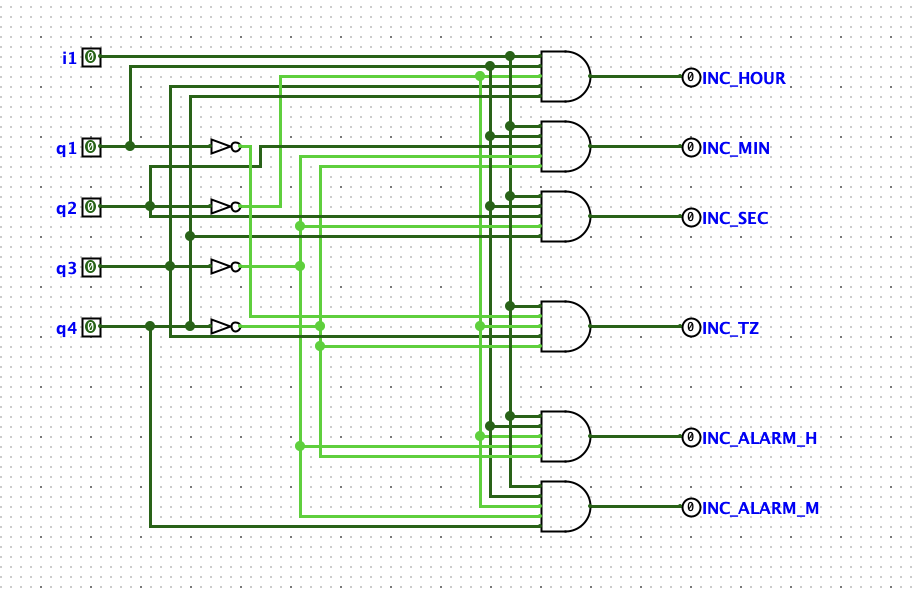
\includegraphics[scale=0.6]{img/21.png}
		\caption{Схема блока Decoder\_i1 }
	\end{figure}
	
	Импульсный сигнал i1 отвечает за увеличение чего-либо на еденицу, блок Decoder\_i1 отвечает за то, чтобы разделять за что отвечает i1 в зависимости от состояния.
	
		\subsection{DisplayMux (Мультиплексор дисплея)}
	Центральный узел управления индикацией. Блок принимает на вход данные от всех источников времени:
	\begin{itemize}
		\item Основные часы (ClockCore);
		\item Блок часовых поясов (TimeZone);
		\item Секундомер (StopWatch);
		\item Будильник (Alarm).
	\end{itemize}
	В зависимости от текущего состояния автомата (\textit{State}), блок коммутирует нужный источник на выход к индикаторам, рисунок \hyperref[disp]{44}. 
	
	\begin{figure}[htpb]
		\centering
		% ЗАМЕНИТЬ ПУТЬ
		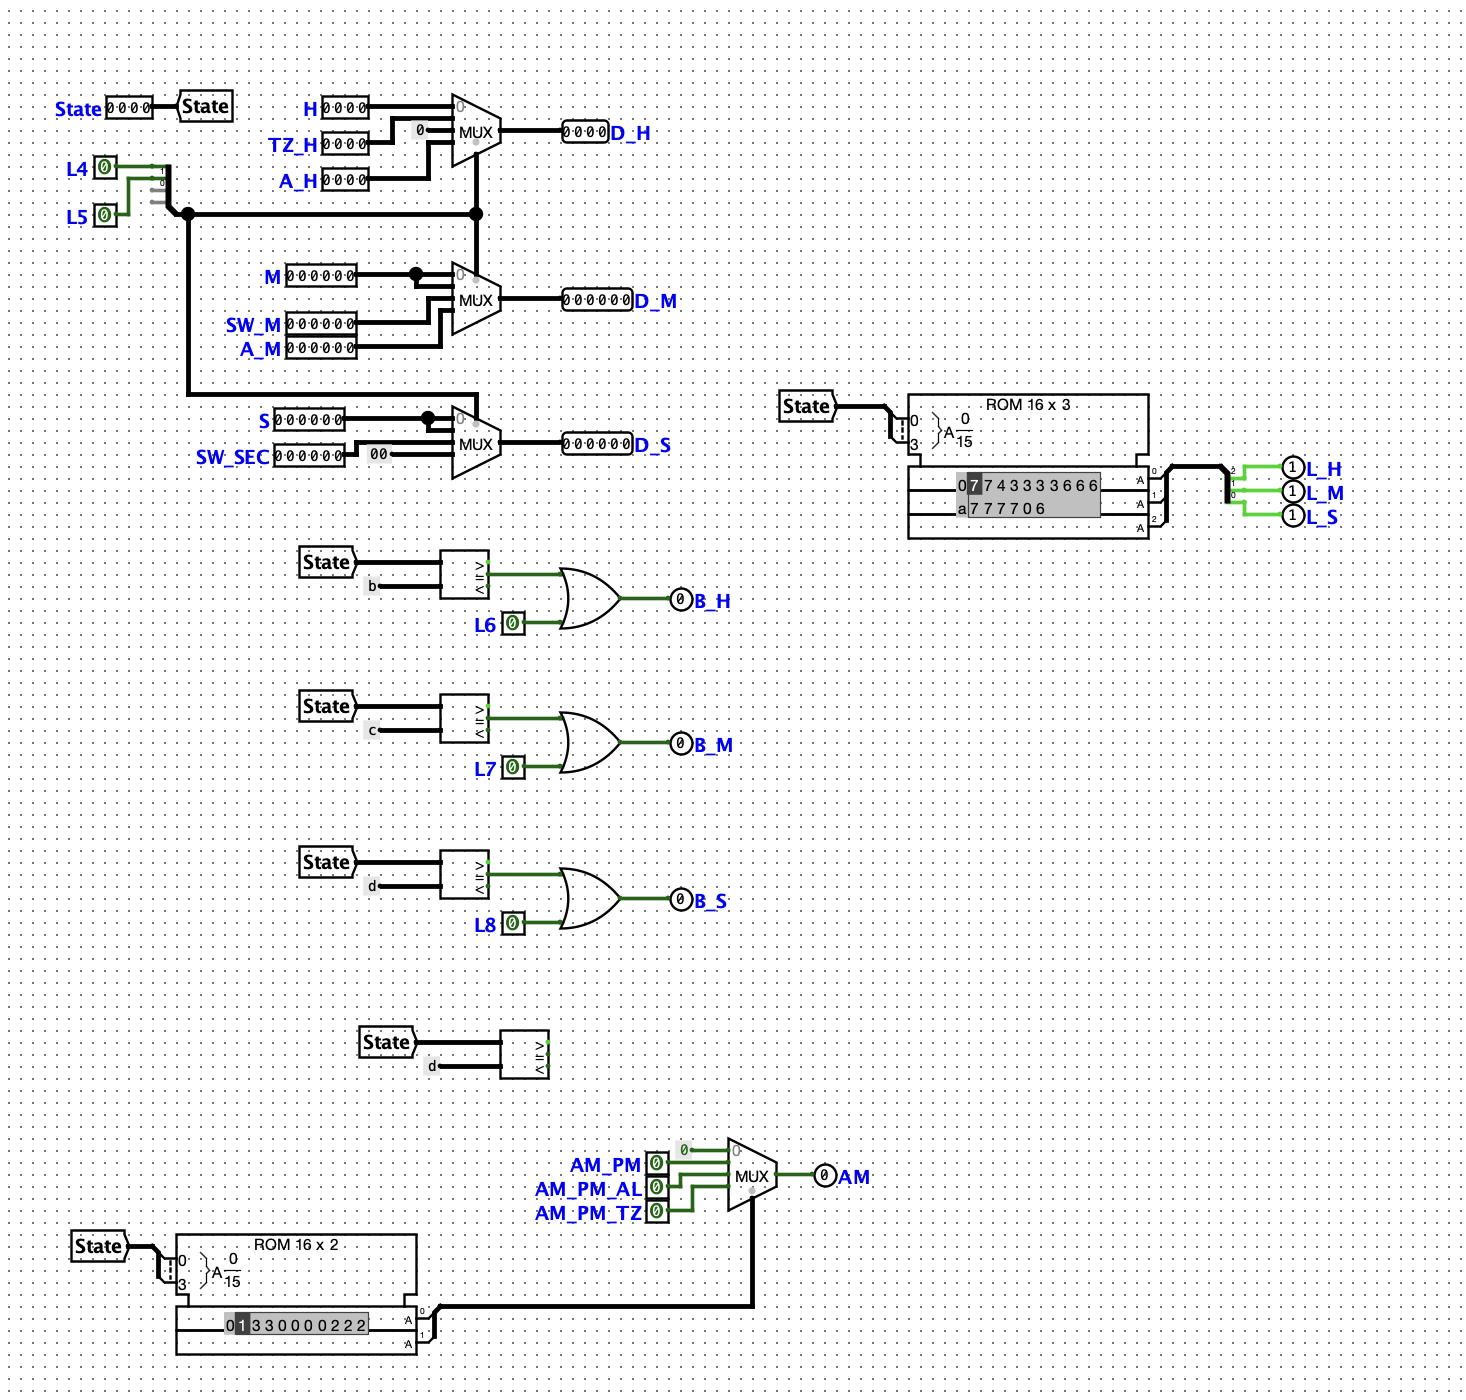
\includegraphics[scale=0.4]{img/33.png}
		\label{disp} 
		\caption{Схема блока DisplayMux}
	\end{figure}
	
	Внутри блока используется ПЗУ для хранения масок отображения (гашение неактивных разрядов) и логика управления миганием при настройке.
	
	\subsection{TimeZone (Блок часового пояса)}
	Блок реализует функцию мирового времени (Вариант B). Содержит:
	\begin{itemize}
		\item 5-битный счетчик для хранения смещения относительно основного времени (0-23 часа).
		\item Арифметический сумматор для вычисления поясного времени.
		\item Логику коррекции переполнения (MOD 12) и инверсии бита AM/PM при переходе через полдень/полночь.
	\end{itemize}
	
	Реализация подсхемы работы разницы часовых поясов на рисунке \hyperref[disp]{45}
	
	\begin{figure}[htpb]
		\centering
		% ЗАМЕНИТЬ ПУТЬ
		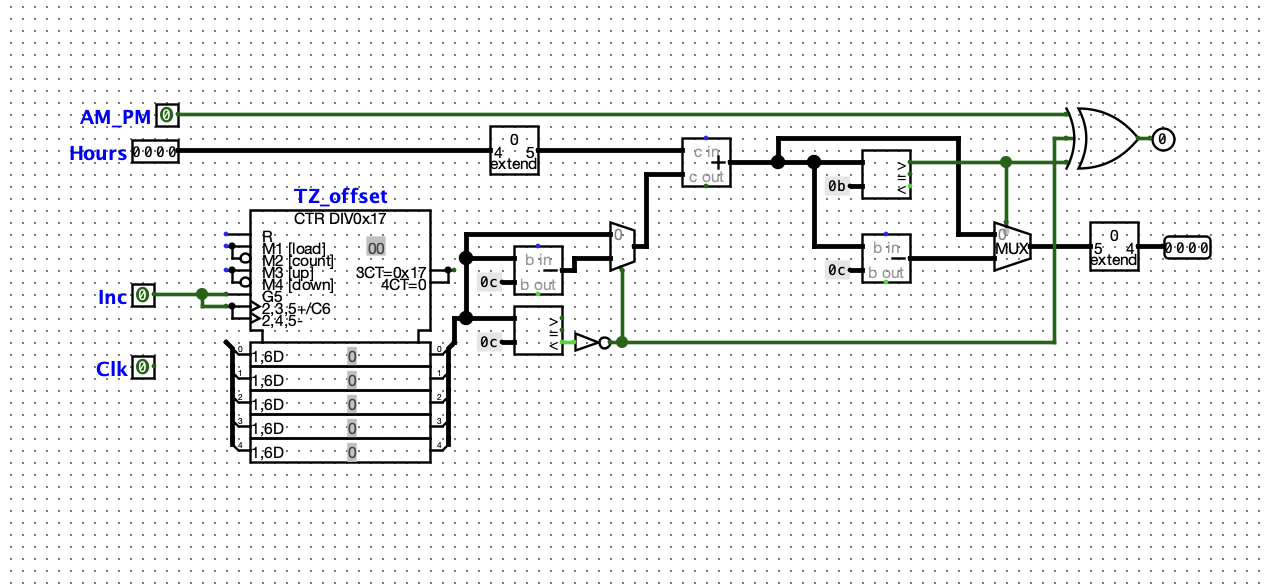
\includegraphics[scale=0.7]{img/25.png}
		\caption{Схема блока TimeZone}
	\end{figure}
	
	\newpage
	\subsection{Alarm (Будильник)}
	Блок реализует функционал будильника с таймером (Вариант I).
	В состав блока входят:
	\begin{itemize}
		\item Регистры памяти (счетчики) для хранения установленного времени срабатывания (часы, минуты).
		\item Схема сравнения (компараторы), проверяющая совпадение текущего времени с установленным.
		\item Таймер длительности сигнала (счетчик до 10), обеспечивающий работу звукового сигнала ровно 10 секунд после срабатывания.
		
		Подсхема будильника в качестве результата отображает заведен ли будильник на текущий момент и сигнал если наступило время будильника рисунок \hyperref[disp]{46}.
		
	\end{itemize}
	
	\begin{figure}[htpb]
		\centering
		% ЗАМЕНИТЬ ПУТЬ
		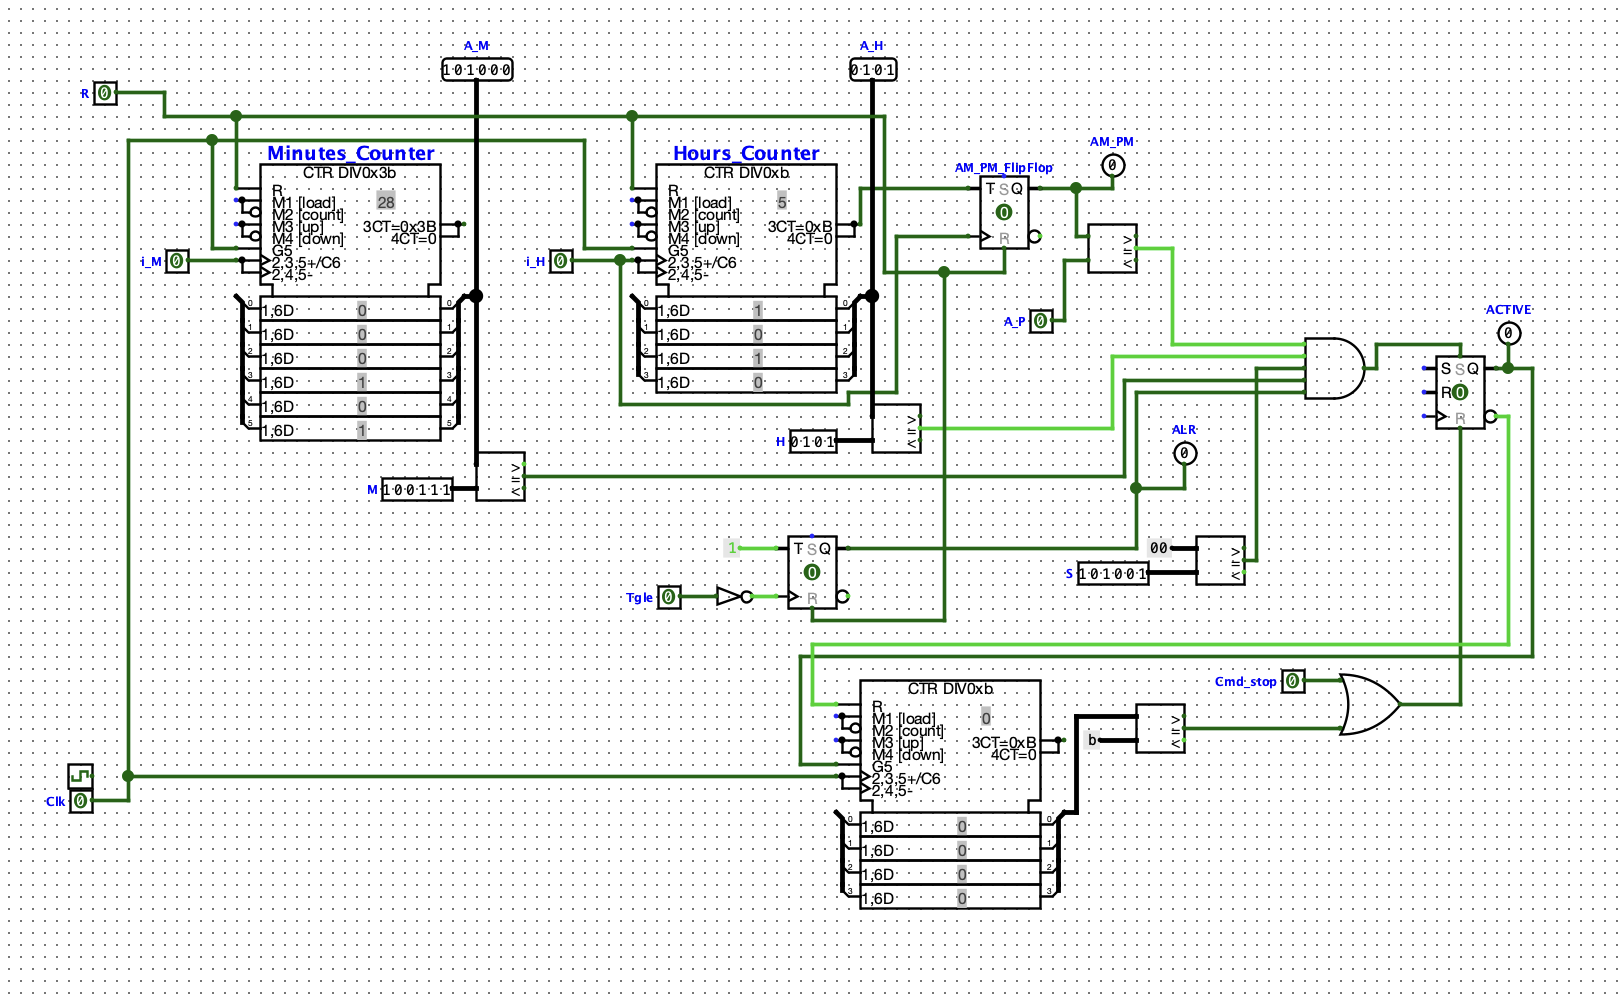
\includegraphics[scale=0.5]{img/24.png}
		\caption{Схема блока Alarm}
	\end{figure}
	
	
	\subsection{Отсчет времени секундомера}
	Данная схема предназначена для отсчета времени секундомера. Она состоит из системы счетчиков.  
	Схема отсчета времени у секундомера представлена на рисунке \hyperref[SW]{47}.
	\begin{figure}[htpb]
		\centering
		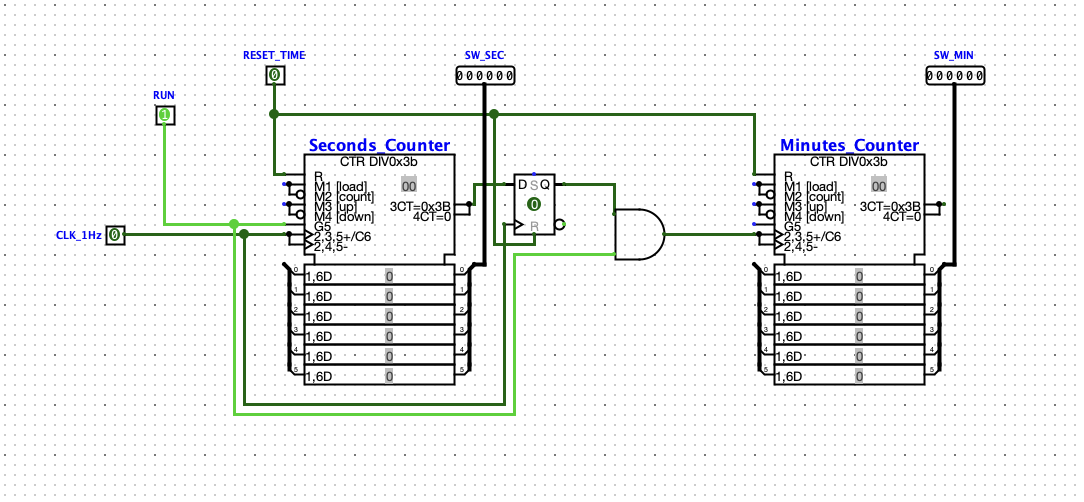
\includegraphics[scale=0.8]{img/13.png}
		\label{SW} 
		\caption{Схема отсчета времени секундомера }
	\end{figure}
	
	\subsection{Звуковая сигнализация}
	Так как в Logisim нет звукового выхода, имитация звуковой сигнализации происходит с помощью светодиода.
	В данной схеме происходит сохранения выходного сигнала каждую четверть часа в течении секунды с помощью D-триггера и счетчика. 
	Схема звуковой сигнализации изображена на рисунке \hyperref[signal]{48}.
	\begin{figure}[htpb]
		\centering
		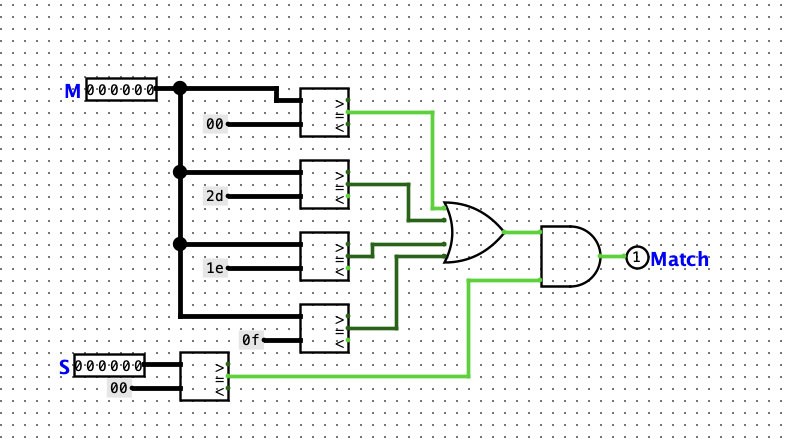
\includegraphics[scale=0.6]{img/14.png}
		\label{signal} 
		\caption{Схема звуковой сигнализации }
	\end{figure}
	
	\subsection{Интерфейс часов}
	Интерфейс часов состоит из 4 индикаторов, отображающих часы и минуты текущего времени, а также минуты и секунды секундомера. Для управления часами присутствуют кнопки <<S>>, <<M>>, <<P>> и кнопка, имитирующая одновременное их нажатие, <<MS>>.
	
	Схема интерфейса электронных часов изображена на рисунке \hyperref[main]{49}.
	\newpage
	\begin{figure}[htpb]
		\centering
		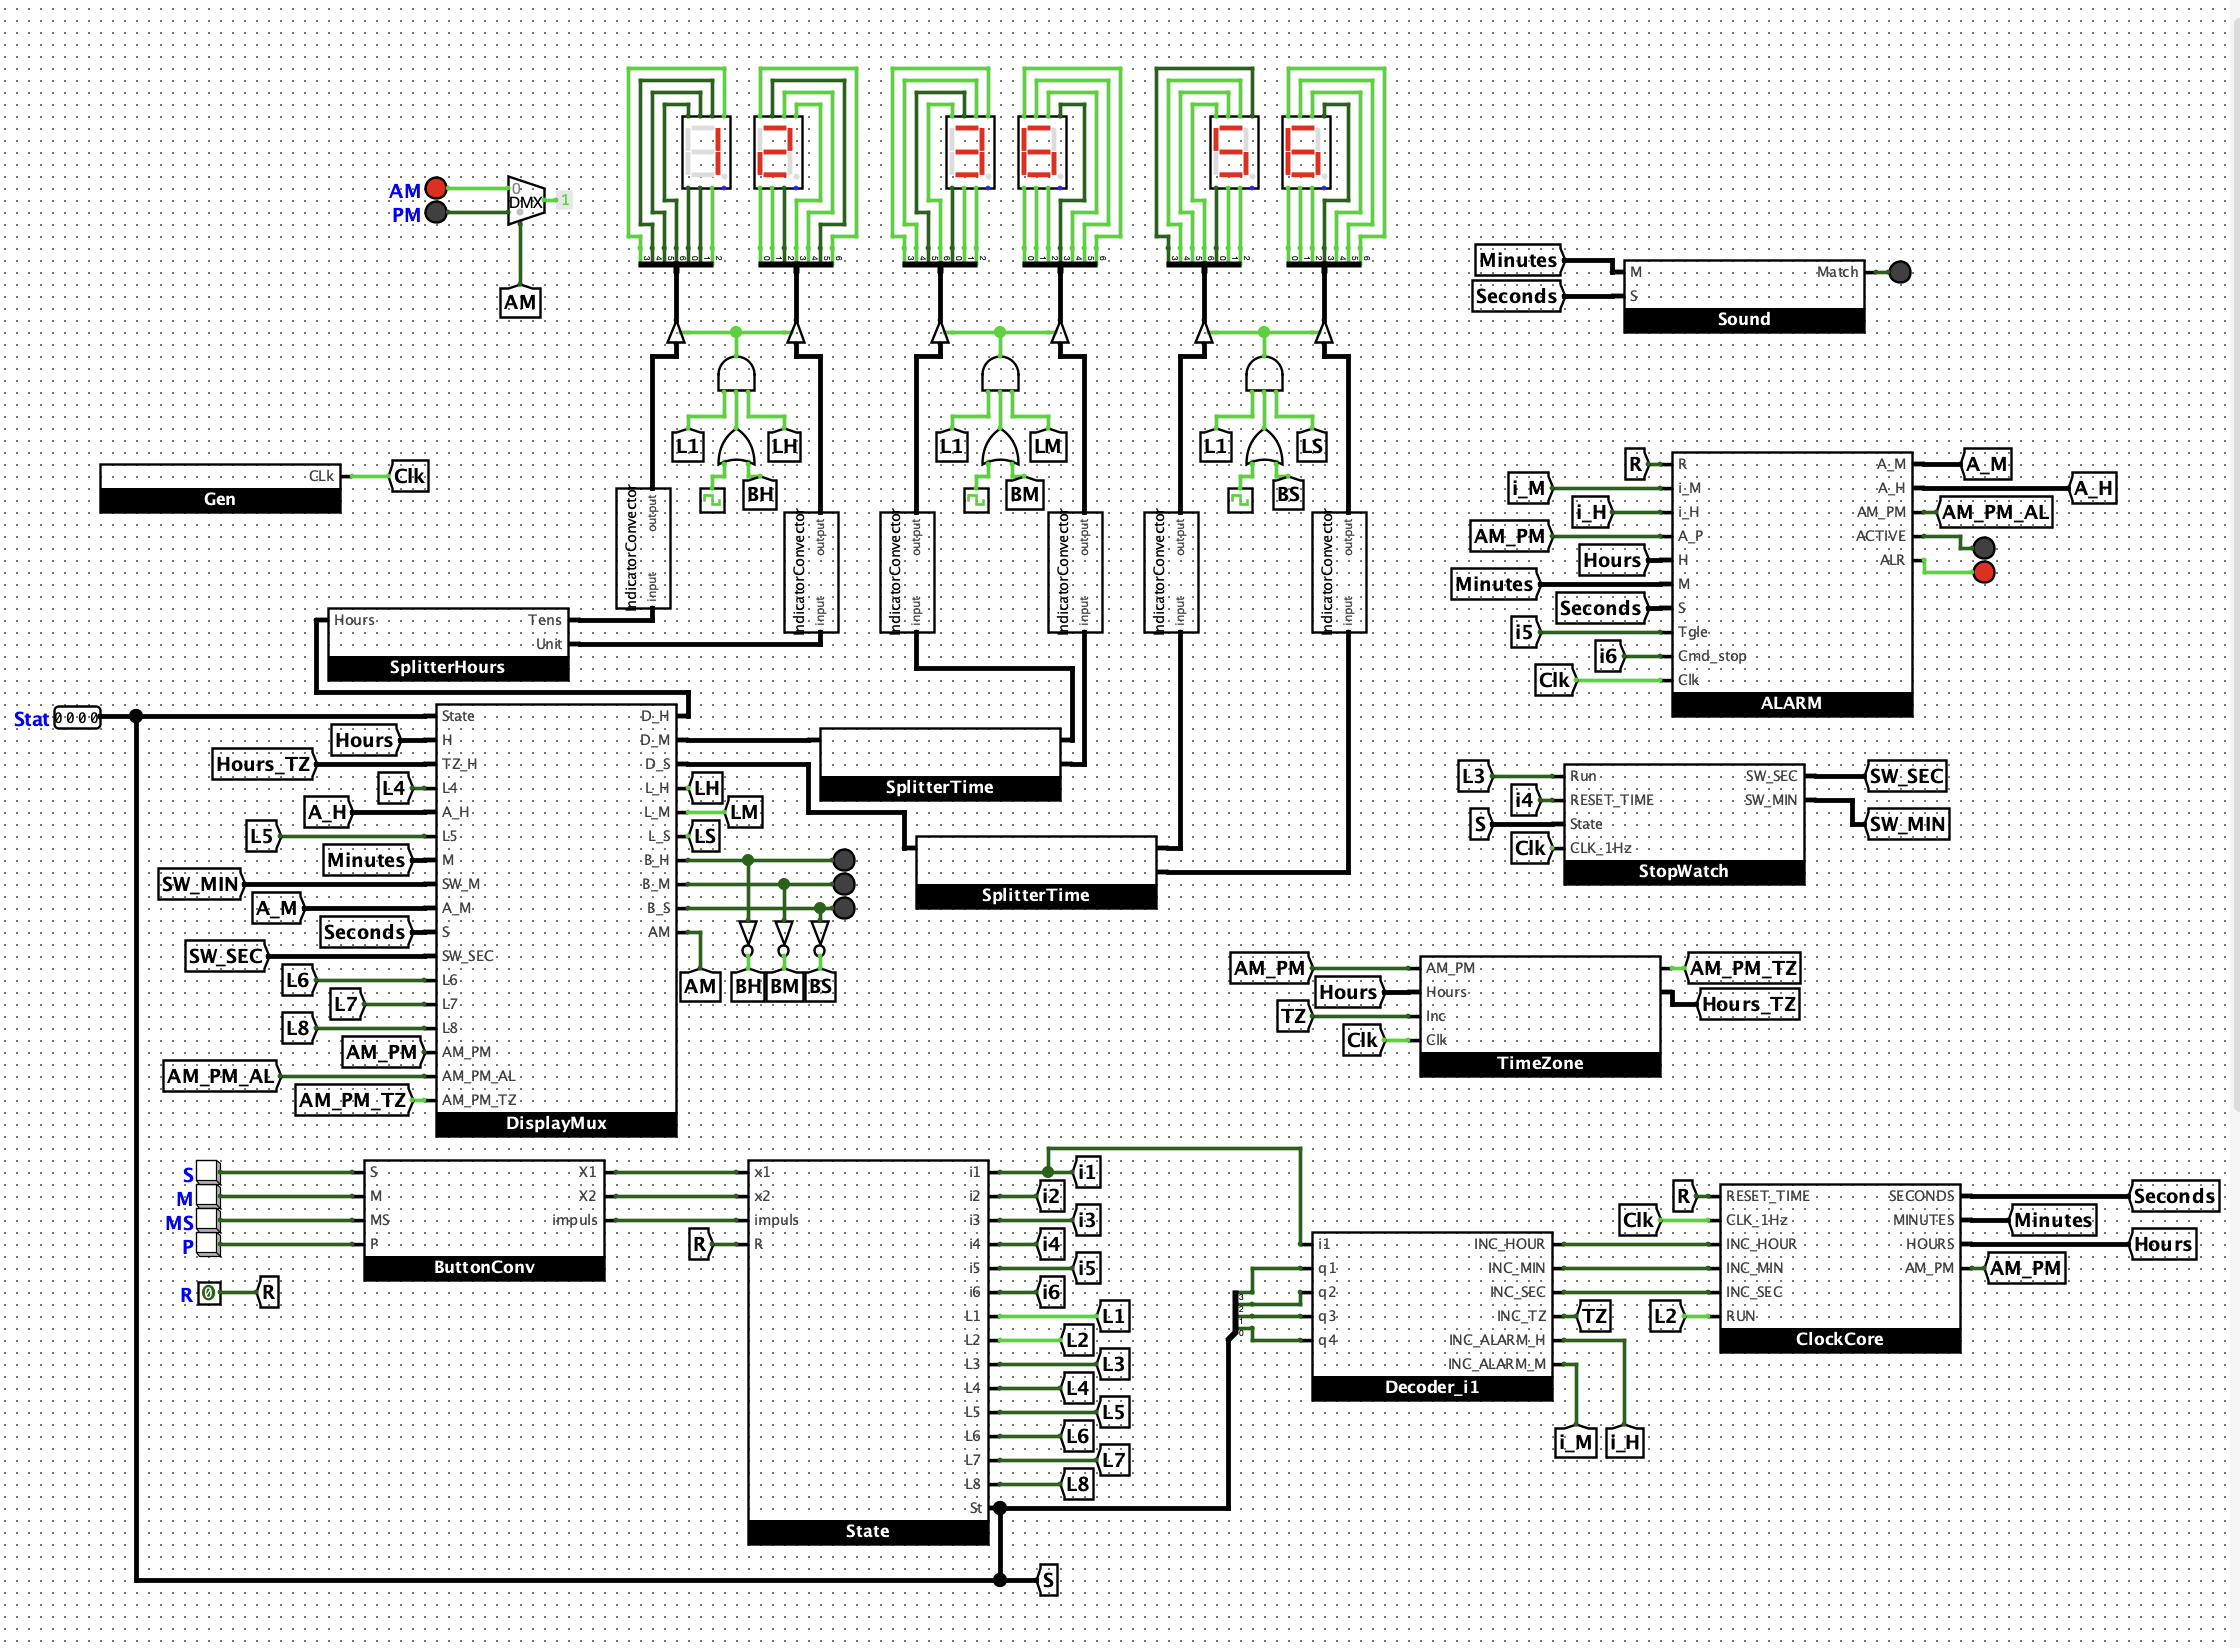
\includegraphics[scale=0.4]{img/27.png}
		\caption{Схема интерфейса электронных часов}
		\label{main} 
	\end{figure}
	
	
	\subsection{Расчет площади схемы}
	Количество компонентов каждого типа на функциональной функциональной схеме электронных часов отображено на рисунке \ref{main} и также перечислены в таблице \ref{tab:stats}.
	\newpage
	\begin{center}
		\captionof{table}{Статистика компонентов схемы}
		\label{tab:stats}
		\begin{tabular}{|l|l|c|c|c|}
			\hline
			\textbf{Компонент} & \textbf{Библиотека} & \textbf{Всего элементов} \\
			\hline
			F & Подсхема & 1 \\
			\hline
			fQ1 & Подсхема & 1 \\
			\hline
			fQ2 & Подсхема & 1 \\
			\hline
			fQ3 & Подсхема & 1 \\
			\hline
			fQ4 & Подсхема & 1 \\
			\hline
			memory & Подсхема & 1 \\
			\hline
			FL & Подсхема & 1 \\
			\hline
			Разветвитель & Проводка & 1 \\
			\hline
			Контакт & Проводка & 86 \\
			\hline
			Тоннель & Проводка & 7 \\
			\hline
			Расширитель битов & Проводка & 1 \\
			\hline
			Элемент НЕ & Элементы & 7 \\
			\hline
			Элемент И & Элементы & 71 \\
			\hline
			Элемент ИЛИ & Элементы  & 13 \\
			\hline
			D триггер & Память & 4 \\
			\hline
			Т триггер & Память & 5 \\
			\hline
			ПЗУ & Память & 3 \\
			\hline
			Счетчик & Память & 7 \\
			\hline
			Мультиплексор & Плексоры & 8 \\
			\hline
			Компоратор & Арифметика & 10 \\
			\hline
			Сумматор & Арифметика & 4 \\
			\hline
			Вычитатор & Арифметика  & 2 \\
			\hline
			\multicolumn{2}{|l|}{\textbf{ВСЕГО (с подсхемами)}} & \textbf{241} \\
			\hline
		\end{tabular}
	\end{center}
	
	\begin{enumerate}[label=]
		\item Непосредственно -- количество компонентов, которые напрямую размещены на главной схеме. Если схема использует вложенные подсхемы, то количество их компонентов не подсчитывается.
		\item Уникальных -- общее количество уникальных компонентов одного типа, включая те, что находятся внутри подсхем. Если подсхема используется несколько раз, то компоненты в ней считаются всего один раз.
		\item Рекурсивно -- полное количество компонентов, включая все из подсхем. Учитываются все экземпляры дублирующихся подсхем.
	\end{enumerate}
	
	Рассчитаем число транзисторов для каждого компонента с учетом количества его вхождений в схему.
	\begin{enumerate}[label=]
		\item $\text{Инвертор: } 4 * 2 = 8$ 
		\item $\text{И: }  6 * 71 = 426$
		\item $\text{ИЛИ: }  6 * 13 = 78$
		\item $\text{Управляемый буфер: }  6 * 11 = 66$
		\item $\text{D-триггер: }  20 * 4 = 80$
		\item $\text{Счетчик: }  16 * 2 * 10 + 16 * 1 * 1 = 336$
		\item $\text{Индикаторный преобразователь: }  400 * 8 = 3600 $
		\item Другие компоненты не требуют транзисторов.
	\end{enumerate}
	Итого получается  $5860$ транзисторов на данную функциональную схему. Исходя из расчета, что на 1 $mm^2$ приходится примерно 1000 транзисторов, функциональная схема реализованных часов будет занимать примерно $5,860 mm^2$.
	
	
	\newpage
	\addcontentsline{toc}{section}{Заключение}
	\section*{Заключение}
	В ходе выполнения лабораторной работы была разработана функциональная схема электронных часов, реализующих следующие функции:
	\begin{itemize}
		\item Отображение и корректировка часов, минут, секунд.
		\item Отображение 2 часовых поясов, разницу которых можно настроить.
		\item 12-часовой формат времени.
		\item Отключение индикаторов с целью экономии электроэнергии.
		\item Останов часов после состояния корректировки текущего времени.
		\item Секундомер с фиксацией накопленного времени и возможностью продолжения отсчета секундомера.
		\item Будильник, играющий 10 секунд, с возвожностью отключения.
		\item Звуковая сигнализация каждые четверть часа в течение секунды.
	\end{itemize}
	
	Для переключения между режимами работы электронных часов используются кнопки <<M>> и <<S>>, а также кнопка имитирующее одновременное  их нажатие -- <<MS>> и кнопка отключающая питание <<P>>.
	
	\noindent Преимущества реализованной функциональной схемы часов:
	\begin{enumerate}
		\item Модульная архитектура. Разделение схемы на независимые блоки обеспечивает легкость отладки и возможность масштабирования.
		\item Погашение неактивных разрядов в зависимости от режима.
		\item Мигание определенных разрядов при корректировке времени.
		\item Работа команд без задержки, благодаря импульсному сигналу и задержке.
	\end{enumerate}
	Недостатки реализованной функциональной схемы часов:
	\begin{enumerate}
		\item Наличие необязательного сигнала i3, так как работа часов возможна без его участия. 
		\item Звуковая сигнализация реализована множеством компараторов, что сильно усложняет возможные доработки, а также лишает пользователя какой-либо вариантивности.
	\end{enumerate}
	Масштабирование: к реализованной функциональной схеме часов можно добавить отображение дня недели или день месяца. Также можно добавить выбор мелодии и вывод букв на дисплей.\\
	
	%\noindent Функциональная схема электронных часов была реализована в Logisim 2.7.1. Схема отображена на \hyperref[func scheme]{рисунке 30} в \hyperref[func scheme]{приложении}.
	
	\newpage
	\section*{Список литературы}
	\addcontentsline{toc}{section}{Список литературы}
	
	\begin{thebibliography}{0}
		\bibitem{tema} Методические указания к курсовой работе [Электронный ресурс]. Сайт секции «Телематика». URL: \href{https://tema.spbstu.ru/userfiles/files/courses/2018-theory-algorithm/KuR_MU.pdf}{https://tema.spbstu.ru/userfiles/files/courses/2018-theory-algorithm/KuR\_MU.pdf} (дата обращения: 12.01.2025).
		\bibitem{karpov} Карпов, Ю. Г. Теория автоматов / Ю. Г. Карпов. – СПб.: Питер, 2003. – 206 с.
		\bibitem{Karno} Карта Карно [Электронный ресурс]. URL: \href{https://sublime.tools/ru/karta-karno}{https://sublime.tools/ru/karta-karno} (дата обращения: 12.01.2025).
	\end{thebibliography}
	
	\newpage
	\phantomsection 
	\addcontentsline{toc}{section}{Приложение}
	\label {func scheme}
	%\includepdf[pages=1,fitpaper]{functional scheme}
	
	
	
	
	\end{document}